\documentclass[journal]{IEEEtran}
% IEEE Robotics and Automation Letters (RA-L) format.
\IEEEoverridecommandlockouts
\usepackage{cite}


%%%% Customized packages
\usepackage[table]{xcolor}
\usepackage{amssymb}
\usepackage{amsmath}
\usepackage{bm}
\usepackage{rotating}
% \usepackage{geometry} % removed: IEEEtran manages page geometry for RA-L
\usepackage[position=bottom]{subfig}
% \usepackage{subcaption}	
% \usepackage{subfigure}
% \usepackage{natbib}
\usepackage{tabularx,booktabs,caption,ragged2e}
\usepackage{graphics, wrapfig}

\DeclareMathOperator{\E}{\mathbb{E}}
\DeclareMathOperator{\R}{\mathbb{R}}
\usepackage{graphicx}

\newcommand{\magpie}{\raisebox{-0.2em}{
\includegraphics[height=1.2em]{magpie.pdf}}}

% hyperref must be loaded last
\usepackage{url}
\usepackage[hidelinks]{hyperref}

\title{\magpie MAGPIE: Multi-Primitive Bimanual Garment Folding from Crumpled States with Pixel-based Flow Matching Policies}


% The \applicant macro works with any number of applicants. There are two
% commands used to separate the names and addresses of multiple
% applicants: \And and \AND.
%
% Using \And between applicants leaves it to LaTeX to determine where to
% break the lines. Using \AND forces a line break at that point. So,
% if LaTeX puts 3 of 4 applicants names on the first line, and the last
% on the second line, try using \AND instead of \And before the third
% applicant name.

% NOTE: applicants will be visible only in the camera-ready and preprint versions (i.e., when using the option 'final' or 'preprint'). 
% 	For the initial submission the applicants will be anonymized.

\author{Halid Abdulrahim Kadi, Houdeyfa Ajrou, Lucy Walsh, Ivan Kapelyukh,
        Kasim Terzi{\'c}, and John Oyekan% <-this % stops a space
\thanks{Manuscript received: \today. This work was supported by the
Engineering and Physical Sciences Research Council, United Kingdom, under
the grant ``A digital COgnitive architecture to achieve Rapid Task
programming and flEXibility in manufacturing robots through human
demonstrations'' (DIGI-CORTEX, EP/W014688/2).}%
\thanks{The authors are with the Department of Computer Science, University
of York; the Department of Computer Science, University of Sheffield; the
Department of Computing, Imperial College London; the School of Computer
Science, University of St Andrews; and the Department of Computer Science,
Loughborough University, United Kingdom. (e-mail:
\texttt{halidkadi.robot@gmail.com}).}%
\thanks{Digital Object Identifier (DOI): see top of this page.}}


\begin{document}

\markboth{IEEE Robotics and Automation Letters. Preprint Version.}%
{Kadi \MakeLowercase{\textit{et al.}}: MAGPIE: Multi-Primitive Bimanual Garment Folding from Crumpled States}

\maketitle
%===============================================================================
%===============================================================================
\begin{abstract}

Garment manipulation remains one of the most challenging task in robotic control due to the large degrees of freedom, severe self-occlusions, and complex underactuated dynamics of the cloth objects. Recent data-driven approaches have demonstrated promising results by fragmenting the garment manipulation pipeline in multi-primitive setups; they typically employ Reinforcement Learning (RL) for flattening and Imitation Learning (IL) or heuristics methods for folding. However, folding garments from arbitrary crumpled configurations within a unified end-to-end learning-based method has remained elusive. We present MEGPIE, a unified, bi-manual, multi-primitive methods that uses flow matching policy for primitive parameter inference. We also proposed central-alignment tasks, where MAGPIE can align a crumpled garment towards arbitrary flattened target position within the workspace; this is especially essential for downstream ironing tasks. Our simulation and real-world experimental results demonstrate that MEGPIE achieves state-of-the-art flattening and folding success rates directly from crumpled states across diverse garments.
\end{abstract}

\begin{IEEEkeywords}
Deformable object manipulation, dual-arm manipulation, imitation learning, flow matching, garment folding.
\end{IEEEkeywords}

\IEEEpeerreviewmaketitle

\section{Introduction}

Robotic manipulation of cloth-like deformable objects presents a significant technical challenge with profound societal and economic implications \cite{kadi2023data}. Automating cloth handling is essential for modernising high-volume industrial garment manufacturing \cite{nayak2018introduction}. It also provides critical assistive care for elderly and mobility-impaired populations \cite{WTOaged2024, disablity2011world, ohneberg2023assistive}, as well as significantly reduces the domestic burden of laundry chores. Moreover, autonomous garment manipulation holds potential in clinical and laboratory settings to minimise contamination risks by safely handling sterile materials \cite{cornish2021clinical}. Despite this broad demand, achieving reliable robotic cloth handling remains exceptionally difficult. Garments possess unique properties that confound traditional control: a high-dimensional state space, severe self-occlusions, and highly underactuated physical dynamics \cite{xue2023unifolding, kadi2023data}. 

Consequently, the garment manipulation literature has historically divided the control pipeline into isolated subtasks: flattening and downstream folding \cite{doumanoglou2016folding}. A pervasive methodological split has emerged to address these distinct phases in the multi-primitive control setup. For flattening, Deep Reinforcement Learning (DRL) is heavily favoured \cite{canberk2022cloth, avigal2022speedfolding, ha2022flingbot, zhou2022aps}; this is because formulating a geometric coverage reward is relatively straightforward, whereas collecting comprehensive human demonstrations across near-infinite crumpled states for Imitation Learning (IL) is intractable. Conversely, for the folding phase, the paradigm flips---formulating a dense RL reward for heavily self-occluded, folded geometries is notoriously difficult \cite{kadi2025lagarnet}, prompting researchers to rely on IL or heuristic template/keypoint-based approaches \cite{barbany2025bifold}. While stitching together these separate policies can yield functional systems \cite{avigal2022speedfolding, canberk2022cloth, xue2023unifolding}, they are inherently brittle; they rely on disjointed classifiers and complex heuristic switching to transition between flattening and folding. Consequently, they lack robustness---if a garment deforms or a fold fails mid-execution, the agent typically cannot autonomously recover or seamlessly switch back to a flattening primitive without resetting the entire pipeline. 


In this paper, we resolve the above challenges through unifying the two process with a multi-primitive imitation learning framework that can be learned in a strict end-to-end manner. Our method, MEGPIE (\textbf{M}ulti-primitiv\textbf{E} \textbf{G}arment manipulation with \textbf{P}ixel-based \textbf{I}mitation l\textbf{E}arning), is a novel data-driven hierarchical framework that robustly unifies flattening and folding for cloth manipulation. MEGPIE bypasses intractable RL exploration by directly cloning human expert strategies and resolve IL's compounding error by learning both \textit{which} behavioural primitive to execute and \textit{how} to continuously parameterise it directly from visual observations. To achieve efficient, stable learning, we ground our policy in Conditioned Optimal Transport Flow Matching (COT-FM) policy \cite{lipman2022flow, black2024pi0, chang2026efficientflow}, mitigating the slow and highly curved inference trajectories of standard diffusion models \cite{chi2025diffusion}. In general, our main contributions are as follows:
\begin{enumerate}
    \item We propose MEGPIE, a unified, end-to-end,  hierarchical data-driven method that robustly bridges the gap between flattening and folding under a single multi-primitive Imitation Learning framework.
    
    \item We synthesise the dual-arm garment manipulation literature with general Parameterised Action Markov Decision Process (PA-MDP) control literature, adapting COT-FM to coordinate both discrete primitive selection and continuous spatial parameter generation while mitigating mode collapse.

    \item We propose central-alignment tasks where the policy flatten and align the garment towards a specific target flattened position around the intersection between dual arms; this is different from conventional cononicalisation alignment tasks \cite{avigal2022speedfolding, xue2023unifolding, canberk2022cloth}.
   
    \item We comprehensively evaluate our system in both simulation and reality, demonstrating that MEGPIE successfully folds a wide variety of previously unseen garment categories and transfers robustly to real-world physical setups in a zero-shot manner.
\end{enumerate}


\section{Related Work}

Learning multi-primitive, dual-arm manipulation for garments requires addressing near-infinite degrees of freedom, dual-arm spatial coordination, and strict workspace constraints. We define garment shaping as a long-horizon, hierarchical process comprising flattening and downstream folding. Note that flattening includes the conventional canonicalisation-alignment tasks \cite{canberk2022cloth} and our proposed central-alignment task. In this section, we reviews dual-arm data-driven shaping methods (Section \ref{sec:dual_arm_shaping}), general multi-primitive control algorithms (Section \ref{sec:multi_primitive_control}), and the evolution of imitation learning policies (Section \ref{sec:diffusion_policies}).

\subsection{Data-driven Approaches in Dual-Arm Garment Manipulation}
\label{sec:dual_arm_shaping}

Data-driven garment manipulation generally falls into two paradigms: learning continuous, low-level end-effector control \cite{black2024pi0, chi2025diffusion, huang2024rekep}, or inferring parameters for predefined behavioural primitives \cite{ha2022flingbot, avigal2022speedfolding}. In this paper, we align with the latter, employing primitives like dual-arm pick-and-fling and pick-and-place to handle the complex dynamics of cloth. Crucially, the choice of state representation significantly impacts policy robustness. While physics-based meshes or dense point clouds are popular \cite{wu2024unigarmentmanip, chen2025metafold}, they are computationally complex to estimate under severe occlusion and often introduce a massive simulation-to-reality gap. Conversely, semantic keypoints provide succinct topological structures \cite{deng2025clasp}, yet often require domain-specific foundation models or structural priors. MEGPIE bypasses these complexities by utilising pure top-down RGB images, inferring semantic structures directly without heavy point-cloud processing or explicit skeleton matching.

\paragraph{Reinforcement Learning for Flattening} Historically, the shaping pipeline has been highly fragmented, with Deep Reinforcement Learning (DRL) dominating the initial flattening phase. Methods like FlingBot \cite{ha2022flingbot}, SpeedFolding \cite{avigal2022speedfolding}, ClothFunnels \cite{canberk2022cloth}, and ClothMate \cite{luo2025clothmate} predominantly employ Spatial Action Value Maps (SAVMs) \cite{lee2021learning} to discretise the action space and select optimal spatial parameters. Because real-world environments impose strict kinematic reachability limits, these methods often mask the action heatmap to prevent self-collisions or utilise active movement strategies—such as dragging or mopping—to pull the garment into the operable workspace \cite{xue2023unifolding}. However, extending SAVM-based DRL to the downstream folding phase is notoriously intractable; the severe self-occlusions inherent to folded geometries create a partially observable state space that fundamentally confounds dense reward formulation.

\paragraph{Imitation Learning for Folding} To overcome the limitations of RL in self-occluded states, the literature pivots heavily to Imitation Learning (IL) \cite{weng2022fabricflownet, kadi2025draper} or heuristic methods \cite{canberk2022cloth} for the folding phase. Systems such as Bifold \cite{barbany2025bifold} and Deng et al. \cite{deng2024learning} generate spatial parameters for folding by relying on step-wise linguistic prompts or predefined keypoint templates. While these IL methods can successfully execute complex folds from perfectly flattened initialisations, they are inherently brittle. Because they operate under the assumption of an already-flattened state, they struggle to recover autonomously if the garment deforms, snags, or shifts mid-execution, requiring a complete manual reset of the pipeline.

\paragraph{Unified Flattening and Folding Systems} Attempts to unify these disparate flattening and folding processes have yielded functional but highly engineered systems. UniFolding \cite{xue2023unifolding} bridges the gap by using dedicated, hard-coded network classifiers to explicitly trigger transitions between flattening primitives (trained via RL) and folding primitives (trained via IL). This rigid phase switching bottlenecks the system's ability to seamlessly mix primitives if a mistake needs correcting mid-fold. Alternatively, UniGarmentManip \cite{wu2024unigarmentmanip} utilises contrastive learning on point clouds to learn cross-deformation structural correspondences, allowing it to replay human demonstrations across different garments. Yet, this demands substantial engineering overhead for skeleton extraction and pre-processing. In contrast, MEGPIE eliminates hard-coded phase classifiers and complex geometric pre-processing, unifying primitive selection and parameterisation in a cohesive, end-to-end visual framework.

\subsection{Data-Driven Multi-Primitive Methods for Manipulation}
\label{sec:multi_primitive_control}

In robotic control, managing complex, long-horizon tasks typically involves decomposing the problem into elemental control modules, or action primitives. The learning paradigms for coordinating these primitives generally fall into two hierarchical frameworks: the Options framework, modelled via Semi-Markov Decision Processes (SMDPs) \cite{sutton1999between}, and Parameterised Action Markov Decision Processes (PA-MDPs) \cite{masson2016reinforcement} (Section \ref{sec:PA-MDP}). Methods grounded in SMDPs concurrently learn both the high-level selection policy and the low-level intra-option motor control. However, learning high-frequency, low-level control modules from scratch for highly deformable objects introduces immense sample complexity. To mitigate this, PA-MDPs have emerged as a robust alternative. By associating predefined, discrete behavioural primitives (e.g., \textit{fling}, \textit{place}) with continuous spatial parameters (e.g., specific x,y,z coordinates and orientations), PA-MDPs abstract away the need to learn low-level motor control from scratch. This makes the framework exceptionally well-suited for dual-arm garment manipulation, where the primary challenge is spatial reasoning rather than trajectory generation.

Within PA-MDPs, DRL approaches have attempted to optimise the joint discrete-continuous action space. Algorithms like MAPLE \cite{nasiriany2022augmenting} utilise hierarchical architectures to evaluate discrete primitive choices alongside their corresponding continuous parameters, while HACMan++ \cite{jiang2024hacman++} extends these principles to 3D point-cloud environments. However, applying online RL to our specific domain presents a critical bottleneck: the combinatorial explosion in the multi-primitive action space. When the discrete choice of primitives is multiplied by the high-dimensional, continuous spatial parameters required for dual-arm coordination across near-infinite crumpled garment states, the state-action space becomes exceptionally vast. In this expanded space, online RL struggles significantly with sample inefficiency, local optima, and an intractable exploration burden.

Consequently, we adopt Imitation Learning (IL) to solve the PA-MDP formulation by leveraging human demonstrations to directly supervise both the discrete selection (which primitive to execute) and the continuous parameterisation (where and how to execute it). Multi-primitive IL approaches, such as HDR-IL \cite{xie2020deep} and PRIME \cite{gao2024prime}, demonstrate that complex sequences can be extracted directly from expert trajectories. However, methods like HDR-IL rely heavily on historical state-action relationships to predict subsequent primitives, while PRIME requires millions of transitions to train an Inverse Dynamics Model (IDM) for parsing demonstrations. In contrast, MEGPIE posits that for highly deformable objects, historical context is less informative than a precise topological estimation of the immediate visual state. Our framework bypasses exhaustive IDM pre-training and historical rollouts, inferring the optimal primitive directly from the current visual observation embedding. This data-driven supervision allows our system to efficiently learn the nuanced visual heuristics that govern multi-primitive transitions, enabling robust garment manipulation without the prohibitive training costs of reinforcement learning.

\subsection{Generative Imitation Learning for Manipulation}
\label{sec:diffusion_policies}

Recent advancements in Behavioural Cloning (BC) have been defined by the integration of generative modelling, which effectively resolves the multimodal action distribution issues that previously limited direct Multi-Layer Perceptron (MLP) methods. While diffusion-like policies \cite{chi2025diffusion} and Action Chunking with Transformers (ACT) \cite{zhao2023learning} excel at continuous end-effector control, their underlying mechanics introduce significant friction in long-horizon, multi-primitive tasks.

Diffusion models conceptualise visuomotor control as conditional trajectory generation dependent on iterative denoising processes \cite{ho2020denoising}. This recursive nature forms highly curved probability trajectories, which translates to slow convergence, high inference latency, and a marked sensitivity to execution noise \cite{black2024pi0}. When these models are deployed for multi-step garment shaping, the compounding latency and execution drift between primitive transitions can severely degrade overall task success. Acceleration strategies, such as DDIM \cite{song2020denoising}, mitigate but do not fully eliminate the reliance on multi-step inference.

Flow Matching \cite{lipman2022flow, chen2023flow} addresses these exact bottlenecks by fundamentally restructuring the generative process. Grounded in optimal transport theory, flow models bypass simulated diffusion paths by directly regressing the vector field of a probability path via Ordinary Differential Equations (ODEs). This direct regression defines straight-line optimal transport flows, substantially reducing the number of required inference steps and offering superior stability and generalisation \cite{zhang2025flowpolicy}. The robotics community has rapidly capitalised on these efficiencies; frameworks such as Flow Policy \cite{zhang2025flowpolicy} have normalised velocity fields conditioned on visual states, while state-of-the-art VLA models like $\pi_0$ \cite{black2024pi0} and $\chi_0$ \cite{yu2026chi_} leverage flow matching to achieve highly reactive, robust physical low-level manipulation.

Despite this success, applying flow-matching policy directly to raw, high-dimensional action spaces can occasionally induce trajectory oscillations, and its application within explicit multi-primitive architectures remains largely unexplored. MEGPIE bridges this gap by directly adapting Conditioned Optimal Transport Flow Matching (COT-FM) to a multi-primitive framework. By constraining the flow generation to output continuous spatial parameters for predefined primitives, MEGPIE demonstrates inference stability. This architectural choice establishes a highly efficient, unified generative policy capable of flattening and folding diverse garments directly from fully crumpled states.


\section{Preliminaries} \label{sec:preliminaries}

We adopt the partially observable Markov decision process (POMDP) \cite{kaelbling1998planning} augmented with action parameterisation \cite{masson2016reinforcement}, collectively referred to as the Parameterised Action POMDP (PA-POMDP, Section \ref{sec:PA-MDP}), as the mathematical formulation for our problem. Specifically, we employ a flow matching policy to infer continuous spatial action parameters across four distinct types of predefined action primitives (Section \ref{sec:action_primitives}). Finally, we describe the Optimal Transport Conditional Flow Matching objective used for policy learning (Section \ref{sec:ot_cfm}).

\subsection{Parameterised Action Partially Observable Markov Decision Process (PA-POMDP)} \label{sec:PA-MDP}

The Partially Observable Markov Decision Process (POMDP) builds upon the standard Markov Decision Process (MDP) \cite{puterman2014markov} by incorporating uncertainty in state observations using the Hidden Markov Model (HMM) framework \cite{rabiner2002tutorial}. An MDP models a stochastic decision system and is formulated as a five-tuple $(\mathcal{S}, \mathcal{A}, \mathcal{P}, \mathcal{R}, \rho_0)$, where $\mathcal{S}$ is the state space, $\mathcal{A}$ is the action space, $\mathcal{P}(s' \mid s, a)$ denotes the transition probability from state $s$ to $s'$ under action $a$, $\mathcal{R}(s, a, s')$ is the reward function, and $\rho_0$ is the initial state distribution. The core attribute of an MDP is the Markov property, whereby the current state $s$ encapsulates all information necessary for the transition and reward functions. A POMDP extends this by assuming the true state $s \in \mathcal{S}$ is not directly observable. Instead, the agent receives observations generated from a latent state via an observation model. Thus, a POMDP is defined as a seven-tuple $(\mathcal{S}, \mathcal{A}, \mathcal{P}, \mathcal{R}, \rho_0, \mathcal{X}, \mathcal{O})$, where $\mathcal{X}$ is the observation space and $\mathcal{O}(x \mid s)$ is the probability of receiving observation $x \in \mathcal{X}$ whilst in state $s$.

In robotics, policies are often developed over a discrete set of action primitives $\Omega$ that enable the robot to perform semantically meaningful behaviours in the environment. Formally, each primitive $\omega \in \Omega$ is represented by a control module $\mathcal{C}_\omega(a^{\omega})$, where $a^{\omega} \in \mathbb{R}^{d_{\omega}}$ signifies the continuous input parameters defined within the parameter dimension $d_{\omega}$. The Parameterised Action MDP (PA-MDP) \cite{masson2016reinforcement} incorporates such action primitives, where the agent selects a parameterised action $a \equiv (\omega, a^{\omega}) \in \mathcal{A}$, comprising the primitive type and its corresponding continuous parameters.

\subsection{Action Primitives} \label{sec:action_primitives}

MAGPIE adopts four types of primitives essential for effective and robust performance: \textbf{TODO: put number of parameters for each.}

\paragraph{Pick-and-Fling:} Primarily utilised for highly crumpled states or garment reorientation, pick-and-fling has proven substantially important for effective flattening. The action easily flips the garment's orientation, reveals hidden key-points, and helps untangle the cloth when needed.

\paragraph{Dual-arm pick-and-place:} Resembling \textit{pick-and-stretch} in ClothMate \cite{luo2025clothmate} and the \textit{fold} primitive in prior literature \cite{xue2023unifolding}, dual-arm pick-and-place adjusts the garment after initial flattening. The primitive is essential for precise folding. To prevent self-collisions, intersecting arm trajectories are executed sequentially.

\paragraph{Single-arm pick-and-place:} Also known as the \textit{drag} primitive, single-arm pick-and-place employs one robot arm to bring the garment toward the intersection of the dual-arm workspace, enabling subsequent flattening and folding. The operation is also vital for fine-grained adjustments, such as aligning trouser legs that fall outside the shared reachable area.

\paragraph{No Operation:} Under this primitive, the robot arms remain stationary, allowing the system to stabilise upon successfully completing the task.

\subsection{Optimal Transport Conditional Flow Matching for Policy Learning} \label{sec:ot_cfm}

Flow matching provides a robust generative framework by constructing continuous-time normalising flows via vector field regression \cite{lipman2022flow}. In the context of robotic policy learning, the objective is to model a conditional action distribution $p_1(a \mid x)$ given an environment observation $x$. To achieve this, Lipman et al. \cite{lipman2022flow} formulate an Ordinary Differential Equation (ODE) that smoothly transports samples from a tractable prior Gaussian noise distribution $p_0$ into the complex, observation-conditioned target data distribution $p_1(\cdot \mid x)$:
\begin{equation}
    \frac{da_k}{dk} = v_\theta(a_k, k \mid x)
\end{equation}
where $v_\theta$ is the learned vector field parameterised by $\theta$ and conditioned on the current observation $x$, and $a_k$ represents the action state at time $k$ \cite{lipman2022flow}. 

Conditional Optimal Transport Flow Matching (COT-CFM) simplifies this objective by sampling the intermediate action $a_k$ from a conditional probability path $p(a_k \mid a_1, k)$ that connects the noise and target distributions. To minimise the transport cost, the optimal path is defined via a deterministic linear interpolant for $k \in [0, 1]$:
\begin{equation}
    a_k = k a_1 + (1 - k) a_0
\end{equation}
This formulation enables the neural network to regress the target vector field without requiring computationally expensive ODE simulation during training. Crucially, the ground-truth instantaneous velocity field, $v_{\text{gt}}(a_k, k)$, is derived directly from the time derivative of this linear interpolant. Because the path between the coupled noise and data samples is a straight line, the ground-truth velocity is simply a constant vector:
\begin{equation}
    v_{\text{gt}}(a_k, k) = \frac{da_k}{dk} = a_1 - a_0
\end{equation}

Substituting this derivation into the formulation yields a highly tractable learning objective. By sampling observation-action pairs $(x, a_1)$ from the expert demonstration dataset $\mathcal{D}$, the network minimises the expected mean squared error between its predicted, observation-conditioned vector field and the straightforward ground-truth velocity:
\begin{equation}
    \mathcal{L}_{\text{FM}} = \mathbb{E}_{\substack{k \sim \mathcal{U}[0,1], \\ a_0 \sim p_0, a_1 \sim \mathcal{D}\\ a_k \sim p(a_k \mid a_1, k)}} \left\| v_\theta(a_k, k \mid x) - v_{\text{gt}}(a_k, k) \right\|^2
\end{equation}

\begin{figure*}[t]
\centering
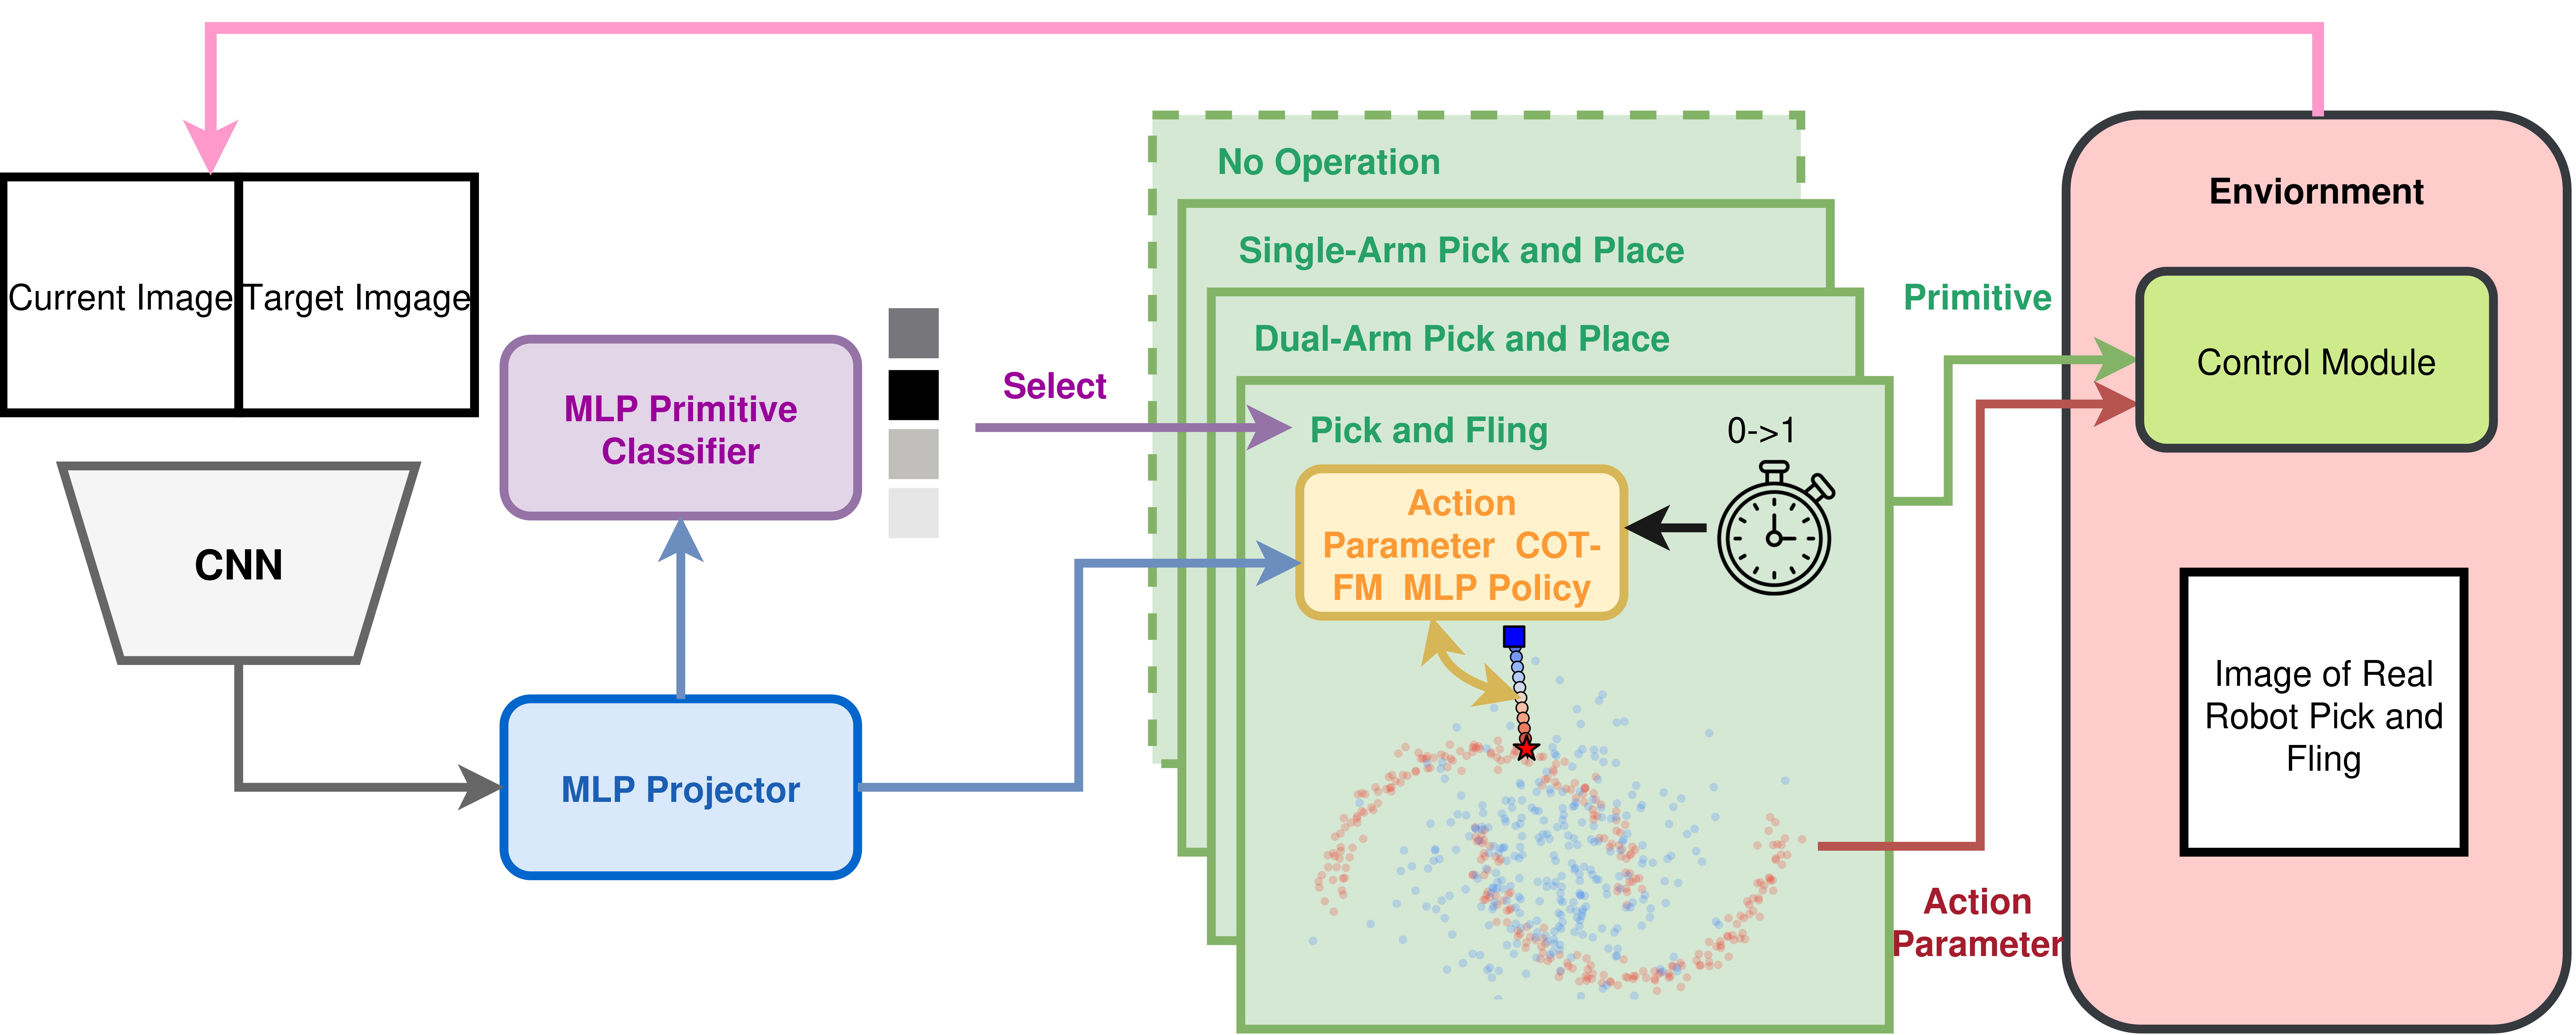
\includegraphics[width=0.98\linewidth]{plots/Magpie-architecture.jpg}
    \caption{The Architecture of MAGPIE. We just snap the resulted action to the corresponding workspace, then snap the pick action on the cloth masks before environment execution.}
        \label{fig:reward-function}
\end{figure*}

\section{Method} \label{sec:method}

We build MAGPIE upon the Parameterised Action Partially Observable Markov Decision Process (PA-POMDP) framework (Section \ref{sec:PA-MDP}). We utilise top-down RGB current and goal images as observations alongside multiple action primitives to execute garment manipulation tasks. An MLP-based classification network predicts the appropriate primitive for the current state (Section \ref{sec:classification}), whilst a suite of primitive-specific Conditioned Optimal Transport Flow-Matching (COT-FM) policies infers the corresponding continuous action parameters (Section \ref{sec:cot_fm_learning}).

To improve learning efficiency, we train MAGPIE using a strategy inspired by Hindsight Experience Replay (HER) \cite{andrychowicz2017hindsight}. Instead of strictly conditioning the policy on the final human-designated goal state—which may be structurally distant from a highly crumpled starting position—we treat intermediate future states within the same trajectory as virtual goals. This transforms partial or incomplete sequences into successful demonstrations of local spatial transformations, providing a dense, reachable learning signal for the policy. Finally, we sequence the flattening and folding behaviours using a vision-based heuristic relying on normalised coverage and alignment Intersection over Union (IoU). The method is developed in simulation and successfully transferred to the real world in a zero-shot manner. Please see Figure \ref{fig:architecture} for an illustration of our method.

% > **Diagram Blueprint for Figure \ref{fig:architecture} (System Architecture)**
% > * **Input Block:** Show a crumpled garment RGB image and a goal folded RGB image ($128 \times 128$) passing through a Shared Vision Encoder (ResNet-18 + GroupNorm).
% > * **Latent Space:** Represent the output passing through an MLP Projector to form the 512-dimensional latent visual embedding $z$.
% > * **Branch 1 (Classification):** Route $z$ to the MLP Classifier. Show a softmax output generating a categorical distribution over 4 primitives (Pick-and-Fling, Dual-arm Place, Single-arm Place, No-Op). Highlight the selected primitive $\omega^*$.
% > * **Branch 2 (Action Parameter Inference):** Create a routing switch controlled by $\omega^*$. The embedding $z$ is routed *only* to the specific MLP-based COT-FM network (e.g., $v_\phi^{\omega^*}$). Show a noise vector $a_0$ iteratively transported over $k=4$ integration steps into the final continuous action parameters $a_1$.

\subsection{Multi-Primitive Learning as Classification}
\label{sec:classification}

Our method, MAGPIE, decouples the high-level primitive selection from the low-level action parameter generation. We employ an MLP-based classification network $f_\theta$ that maps the latent state $z$ to a predicted primitive $\omega = \arg\max_k f_{\theta}(z)_k$. To address the severe imbalance between demonstrated primitives in our dataset, we optimise the network using a weighted cross-entropy loss:
$$\mathcal{L}_{cls}(\theta) = - \sum_{\omega \in \Omega} \lambda_\omega y_\omega \log(\hat{y}_\omega)$$
where $y_\omega \in \{0, 1\}$ is the ground-truth binary indicator for primitive $\omega$, $\hat{y}_\omega$ is the predicted probability from the network, and $\lambda_\omega$ denotes the empirical class weight used to penalise majority classes. 

Once the optimal primitive $\omega^*$ is identified, the system must determine the precise spatial execution parameters. To ensure a smooth transition from discrete reasoning to continuous generation, the latent visual embedding $z$ is routed exclusively to the designated generative network corresponding to $\omega^*$. Detailed architectural specifications for this classification network are provided in Appendix \ref{app:architecture}.

\subsection{Primitive Parameter Learning via COT-FM Policy}
\label{sec:cot_fm_learning}

We utilise Conditioned Optimal Transport Flow Matching (COT-FM) \cite{black2024pi0, lipman2022flow, liu2022rectified} (detailed in Section \ref{sec:ot_cfm}) to model the generative mapping from an initial noise distribution to the target action parameter distribution. Rather than employing a single one-size-fits-all network conditioned on a one-hot encoding, we instantiate independent vector field networks $v_{\phi}^{\omega}$ for each primitive type $\omega \in \Omega$. This architectural split effectively prevents mode collapse and parameter interference across distinctly different robotic behaviours. We demonstrate the empirical superiority of this decoupled approach via ablation studies in our experiments section.

Building upon the optimal transport formulation defined in Section \ref{sec:ot_cfm}, the specific vector field network $v_{\phi}^{\omega}(a_k^\omega, k \mid z)$ for the selected primitive $\omega$ is trained to regress the constant target velocity $u_k = a_1 - a_0$. We optimise this via the following conditional flow matching objective:
$$\mathcal{L}_{para}^{\omega}(\phi) = \mathbb{E}_{\substack{k \sim \mathcal{U}[0,1] \\ a_0 \sim \mathcal{N}(\bm{0}, \bm{I}) \\ a_1 \sim \mathcal{D}^\omega}} \left[ \| v_{\phi}^{\omega}(a_k^\omega, k \mid z) - (a_1 - a_0) \|^2 \right]$$
where $\mathcal{D}$ represents the expert demonstration dataset where primitive $\omega$ was executed. The exact implementation details of these policy networks are given in Appendix \ref{app:architecture}.

% \subsection{Representation Learning via Semantic Keypoints}
% \label{sec:representation_learning}

% Unlike dense point clouds or complex meshes, semantic keypoints carry explicit semantic meaning and can be intuitively described using natural language. As noted by Deng et al. \cite{deng2025clasp}, they "offer a more sparse and succinct representation and focus on distinct structural features of clothes like sleeves and shoulders." 

% Because different garment categories possess varying topological structures, the number of semantic keypoints differs across items (e.g., long-sleeve shirts typically have 15, trousers 8, skirts 7, and dresses up to 17). To accommodate this variance within a static network architecture, we fix the output dimension of the semantic keypoint regression head to $17 \times 2 = 34$, and pad non-effective entries for simpler garments with a placeholder value of $-1$. 

% Furthermore, while our simulation environment allows for automatic keypoint annotation via deprojection from flattened states, physical real-world data lacks these privileged labels. Consequently, each dataset trajectory is marked with a domain flag. The semantic keypoint loss is exclusively computed on simulation data; for real-world batches, the gradients from this representation head are masked out entirely.

% For each step, a CNN-based encoder $e_{\theta}$ processes the image observation $x$ into a latent representation $z_t$. To promote geometrically meaningful embeddings that overcome the severe self-occlusion issues inherent to cloth manipulation, we train $e_{\theta}$ jointly with an auxiliary linear regression head $s_{\vartheta}$ to predict the privileged semantic keypoints $s$, trained via the Mean Squared Error (MSE) loss:
% $$\mathcal{L}_{rep} = \frac{1}{B_{sim}}\sum_{i=1}^{B_{sim}} \| s_{\vartheta}(z_i) - s_i \|^2$$
% The shared encoder weights are thus holistically shaped by gradients flowing from both the flow-matching policy networks and the structural representation loss. The exact network architecture is given in Appendix \ref{app:architecture}.

% \begin{figure}[!t]
%     \centering
%     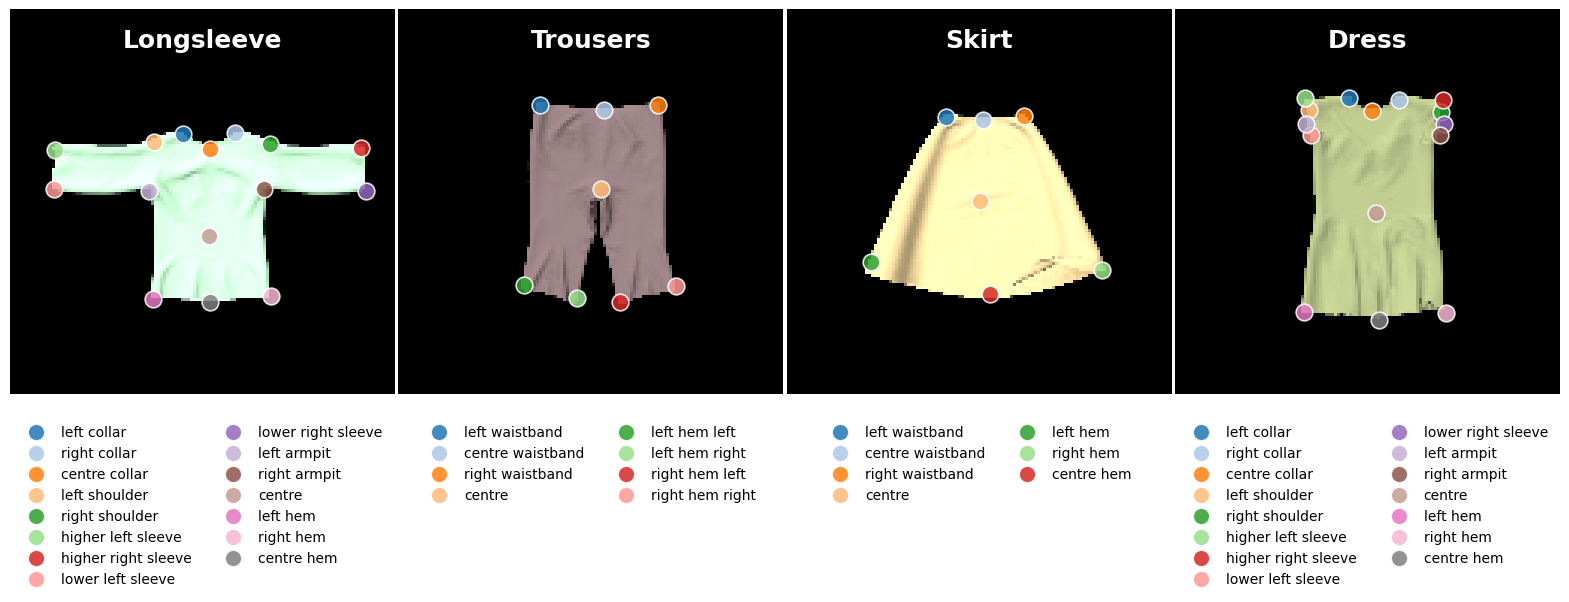
\includegraphics[width=1.0\linewidth]{plots/flattened_garments_semkey_plot.png}
%     \caption{Semantic Keypoints for Different Garment Types. The interface highlights the core topological structures utilised for representation learning. \textbf{PLACEHOLDER: update the image and add take away message.}}
%     \label{fig:semantic_keypoints}
% \end{figure}

% We manually annotate a set of semantic keypoints in simulation on each garment mesh using a clickable image-based interface (as visualised in Figure \ref{fig:semantic_keypoints}). Each clicked pixel is deprojected into the 3D world frame using the known camera parameters. The semantic keypoint is then assigned to the particle whose Euclidean distance to the deprojected point $\mathbf{x} \in \mathbb{R}^3$ is minimal:
% $$k = \arg\min_{i} \lVert \mathbf{p}_i - \mathbf{x} \rVert_2$$
% This procedure yields an approximate but consistent semantic correspondence across time, heavily inspired by recent advancements in semantic keypoint tracking \cite{deng2025clasp}.


\subsection{Data Augmentation and Future-State Goal Sampling}
\begin{figure}
    \centering
    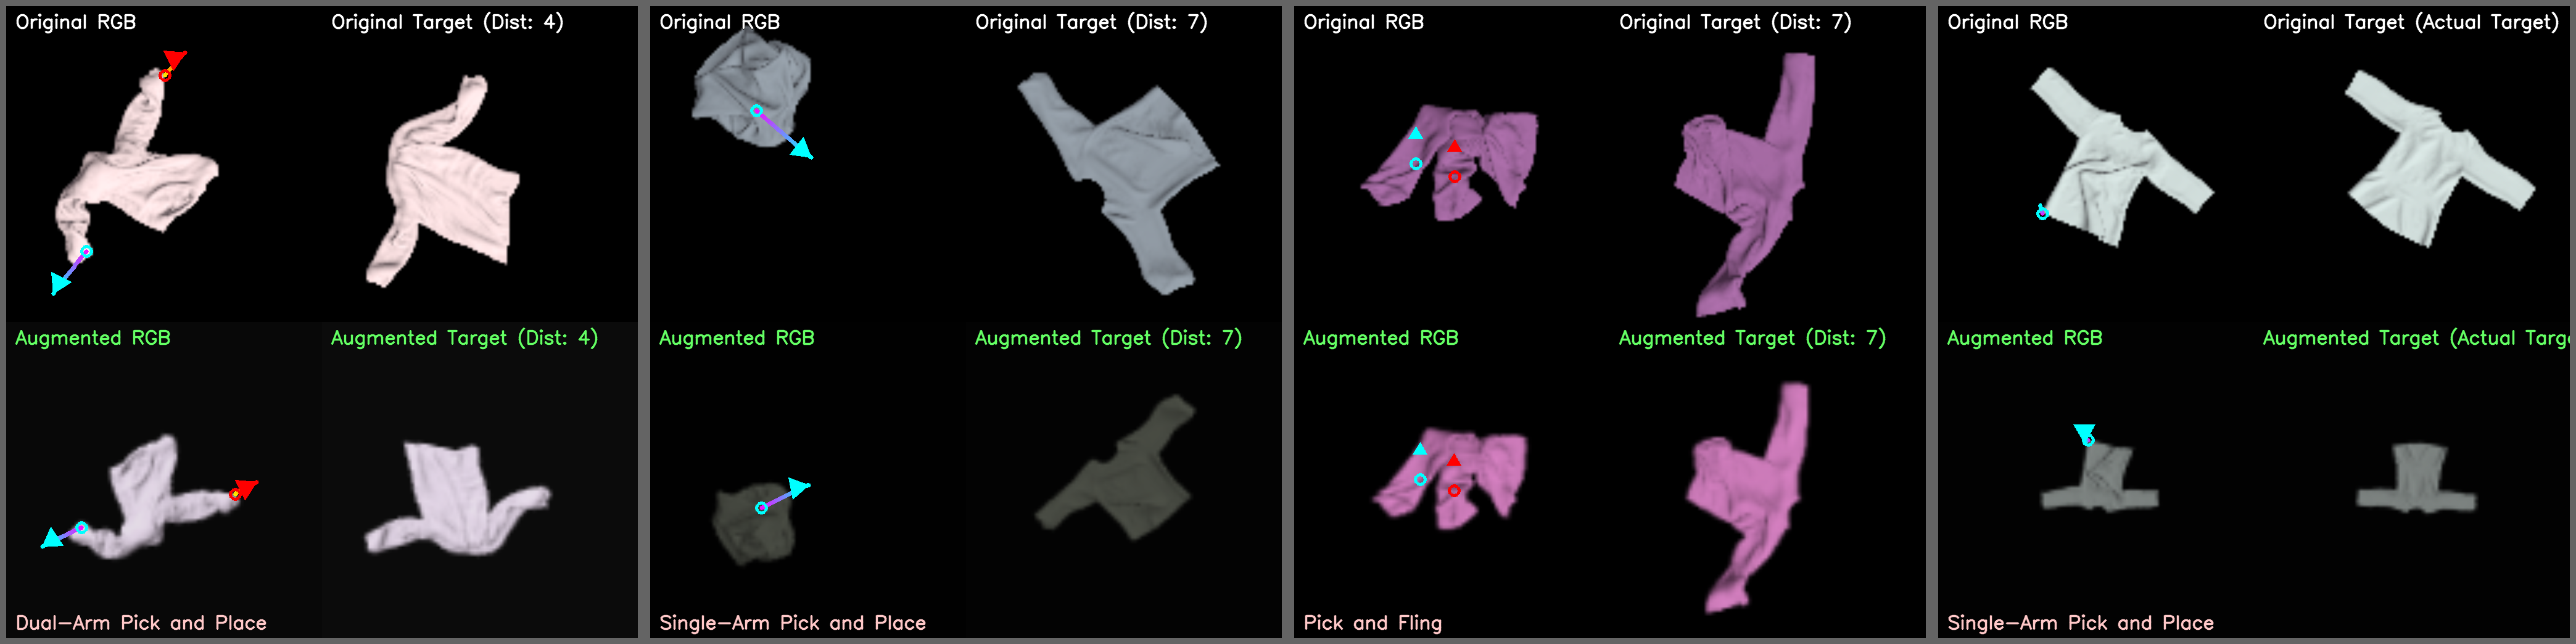
\includegraphics[width=1.0\linewidth]{plots/dataloader_augment_master_multi_batch.png}
    \caption{Data Sampling and Augmentation. The data augmentation includes rotation, flipping, scaling and colour jittering, RGB channel permutation as well as gripper-swapping. The hindsight sampling randomly select the target states as well as the actual target of the trajecotory.}
    \label{fig:placeholder}
\end{figure}
To improve data efficiency and provide a dense, reachable learning signal, we actively sample future states for goal conditioning during training. Rather than conditioning the policy strictly on the terminal goal state of an episode, we dynamically sample a future observation $x_{goal}$ from a randomly selected future time step $t + \Delta t$ within the same trajectory sequence. This acts as a proximal sub-goal, effectively bridging the severe visual distribution shift between highly crumpled initial states and perfectly folded final states. By anchoring the generative policy to near-term geometric changes, the network learns local spatial transformations much faster. This future-state relabelling is directly inspired by Hindsight Experience Replay (HER)~\cite{andrychowicz2017hindsight}, which similarly converts partial rollouts into successful goal-reaching demonstrations.

Furthermore, to ensure robustness to visual perturbations and bridge the simulation-to-reality gap, we apply an aggressive suite of spatial and visual data augmentations to the RGB observations prior to latent encoding. These include color jittering (modifying brightness, contrast, saturation, and hue), random channel permutation, random vertical flipping (with corresponding inversions of spatial action coordinates), random scaling within a $[0.7, 1.0]$ range, and random rotations in $1^\circ$ increments. To handle the symmetrical nature of dual-arm manipulation, we also employ an action-swapping augmentation with a $50\%$ probability, which geometrically mirrors the observation and remaps the corresponding left/right arm action parameters.

\subsection{Training Details}
All network components—including the shared visual encoder, the primitive classification network, and the suite of flow-matching action generative models—are optimised jointly in an end-to-end manner. The overall training objective is formulated as a weighted sum of the primitive classification loss $\mathcal{L}_{prim}$ and the sum of the optimal transport flow-matching losses across all active primitive networks $\sum_{\omega \in \Omega} \mathcal{L}_{para}^{\omega}$:
$$\mathcal{L}_{total} = \beta_{prim} \mathcal{L}_{prim} + \beta_{para} \sum_{\omega \in \Omega} \mathcal{L}_{para}^{\omega}$$
where the scaling coefficients are empirically set to $\beta_{prim} = 0.01$ and $\beta_{para} = 1.0$ to balance the objectives. We employ the AdamW optimiser and apply weighted cross-entropy to handle the highly imbalanced distribution of primitives within the demonstration dataset. 

Our dataset comprises 200 simulation episodes for each garment category, and 40 real-world episodes for each physical garment instance. Each episode is rolled out to a maximum of 20 steps. A complete and detailed breakdown of all hyperparameters, network architectures (including hidden dimensions and normalisation layers), and environment configurations can be found in Appendix \ref{app:architecture}.

\begin{figure}[!t]
    \centering
    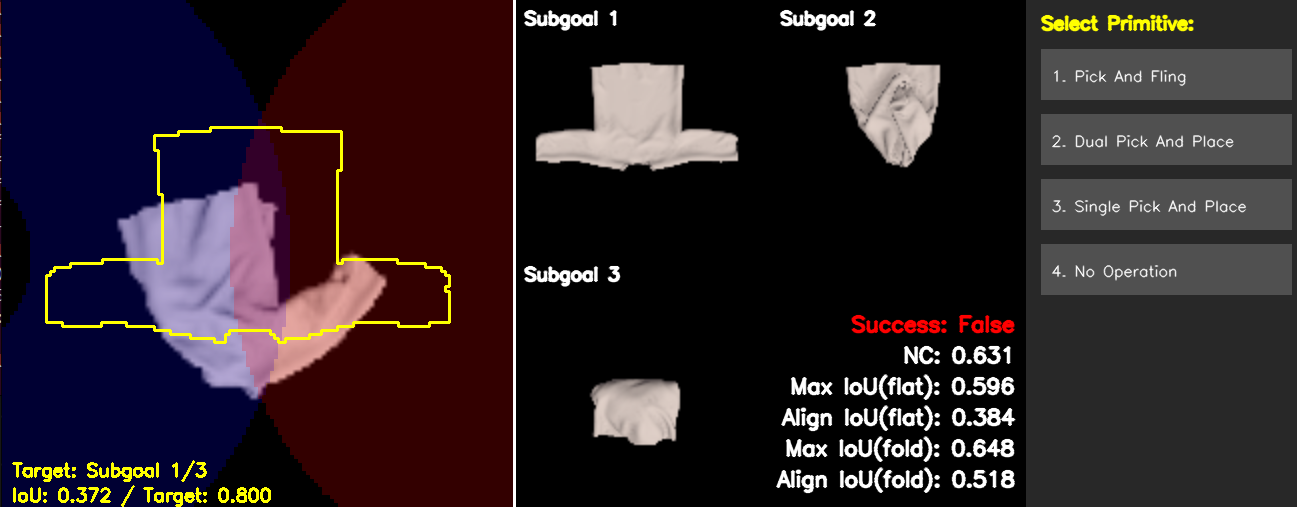
\includegraphics[width=0.49\linewidth]{plots/human-interface-initial.png}
    \hfill
    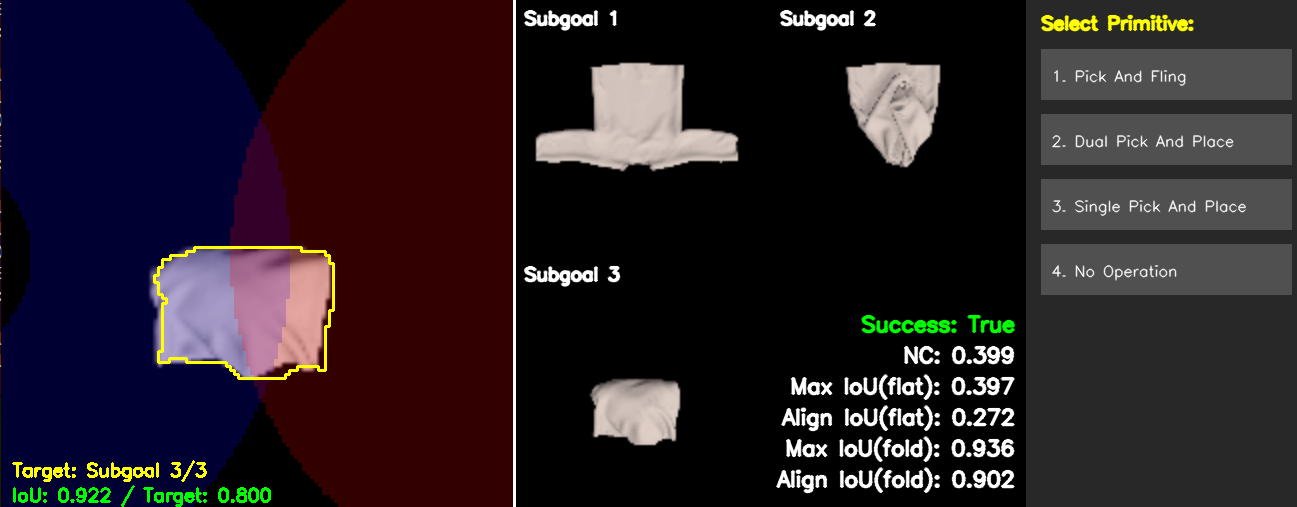
\includegraphics[width=0.49\linewidth]{plots/human-interface-success.png}
    \caption{Interface that is used to collect human demonstration data and human baseline evaluation}
    \label{fig:qualitative_sota_canon}
\end{figure}


\begin{figure}[!t]
    \centering
    % \includegraphics[width=0.5\linewidth]{plots/your_figure.png}
    \caption{Data Augmentation and Sampling}
    \label{fig:placeholder}
\end{figure}

\section{Experiments}
\label{sec:experiments}

We develop our proposed method MAGPIE based on the decoupled multi-primitive architecture and the underlying Paremeterised Action Partially Observable Markove Decision Process (PA-POMDP) framework introduced in Section \ref{sec:preliminaries}. By separating discrete primitive classification from continuous parameter generation via the  Conditioned Optimal Transport Flow-Matching (COT-FM) policy \ref{sec:cot_fm_learning}, MAGPIE aims to isolate distinct robotic behaviours and bypass the learning instabilities common to unified pixel-to-action generative models. In this section, we perform a rigorous empirical evaluation of MAGPIE in both simulation and the real world. Our experimental evaluation is designed to answer the following core research questions:

\paragraph{RQ1 (Section \ref{sec:exp_sota}):} How does MAGPIE compare to state-of-the-art (SoTA) domain-specific flattening and folding baselines under similar observational and action constraints? 

\paragraph{RQ2 (Section \ref{sec:exp_abl}):} What is the individual contribution of MAGPIE's architectural components, including the decoupling layout on primitive-parameter inference, the continuous action-parameter network backbone, and the composition of the training dataset?

\paragraph{RQ3 (Section \ref{sec:exp_real_world}):} How effectively does the simulation-trained MAGPIE policy transfer to real-world physical deployments?

\subsection{Comparison Against SoTA Garment Manipulation Systems}
\label{sec:exp_sota}

In this set of experiments, we benchmark MAGPIE against leading domain-specific garment-manipulation multi-primitive approaches in simulation. For non-unified baselines, we evaluate ClothFunnels \cite{canberk2022cloth} and ClothMate \cite{luo2025clothmate}. For unified framework baselines, we compare against UniFolding \cite{xue2023unifolding}. To ensure a fair comparison, we exclude methods that rely on step-wise language instructions.

\paragraph{Simulation Experimental Setup}
We evaluate MAGPIE across both simulation and physical domains. We build our simulation environment upon the ClothFunnels variant of the SoftGym benchmark \cite{lin2020softgym}, powered by the PyFlex physics engine \cite{li2018learning}. We source realistic garment meshes from the Cloth3D dataset \cite{bertiche2020cloth3d}, specifically selecting long-sleeve T-shirts, trousers, skirts, and dresses. For each category, our dataset comprises 200 training episodes, 30 validation episodes, and 30 evaluation episodes. To ensure robust policy learning, we utilise a diverse split of ``hard'' (highly crumpled with severe self-occlusion) and ``easy'' (semi-flattened) initial states, directly following the ClothFunnels methodology. Specifically, the 200 training trials use a mixture of ``hard'' and ``easy'' configurations, whereas the validation and evaluation trials strictly use ``hard'' initialisations.  We preserve most parameter distributions from the original ClothFunnels environment, where a top-down camera observes the centre of the world frame. However, for our novel central-alignment and folding tasks, we explicitly align simulation properties with our real-world setup. This includes matching workspace radii, dual-arm base placements, and camera configurations to mirror our physical hardware cell. Furthermore, we adjust fabric stiffness values and cloth particle radii to emulate realistic garment dynamics. A side-by-side comparison of these environmental parameters is detailed in Table \ref{tab:sim-real-params}. Detailed mechanics of the simulation physics, mesh rendering, and primitive trajectory parameters are deferred to Appendix \ref{app:simulation_details}. We set all the evaluation step strictly as 20---there is no early stopping at the success states.

\begin{table*}[!t]
\caption{Comparison of physical and simulated environmental parameters, highlighting the reduced sim-to-real gap in our experimental framework.}
\label{tab:sim-real-params}
\centering
\small
\begin{tabular}{l|cc}
\toprule
\textbf{Parameter} & \textbf{ClothFunnels} & \textbf{Ours} \\
\midrule
Camera Height & $2.0\,\mathrm{m}$ & $1.65\,\mathrm{m}$ \\
Camera FoV  & 45x45 & 69x42 \\
Camera Resolution  & 480x480& 1280x720 \\
Particle Radius & $0.0140\,\mathrm{m}$ & $0.0175\,\mathrm{m}$ \\
Cloth Stiffness & (0.75, 0.02, 0.02) & (0.8, 0.6, 0.8) \\
Arm Base Distance & $1.765\,\mathrm{m}$ & $1.2\,\mathrm{m}$ \\
Arm Workspace Radius & $(0\,\mathrm{m}, 1.5\,\mathrm{m}), (0\,\mathrm{m}, 1.5\,\mathrm{m})$ & $(0.1\,\mathrm{m}, 0.85\,\mathrm{m}), (0.25\,\mathrm{m}, 0.9\,\mathrm{m})$ \\
\bottomrule
\end{tabular}
\end{table*}

\paragraph{Metrics for Canonicalisation and Central Alignment Tasks in Simulation}
For all continuous flattening metrics, we report the final value achieved at the end of the trajectory (capped at 20 steps):
\begin{enumerate}
    \item \textbf{Normalised Coverage (NC):} The ratio of the garment's current 2D projected area to its maximally flattened area, bounded in $[0, 1]$.
    \item \textbf{Normalised Improvement (NI):} The relative coverage increase from the initial state, defined as $\text{clip}(\frac{c_t - c_0}{c_{\text{max}} - c_0}, 0, 1)$.
    \item \textbf{Alignment Intersection-over-Union (A-IoU):} The IoU overlap between the current garment segmentation mask and the target goal mask.
    \item \textbf{Success Rate (SR):} The percentage of trials simultaneously achieving $\text{NC} > 80\%$ and $\text{A-IoU} > 70\%$; we report both cross-trajectory success rate (C-SR) and last step success rate (LS-SR).
\end{enumerate}

\paragraph{Metrics for Folding in Simulation}
In simulation, we evaluate folding using fine-grained, particle-based geometric distances alongside vision-based metrics:
\begin{enumerate}
    \item \textbf{Mean Particle Distance (MPD):} We apply rigid Procrustes alignment between the current ($\{\mathbf{p}_t^i\}_{i=1}^N$) and goal ($\{\mathbf{p}_g^i\}_{i=1}^N$) particle sets via Singular Value Decomposition (SVD) on centred point clouds to ensure translational and rotational invariance \cite{canberk2022cloth}.
    \item \textbf{Mean Keypoint Distance (MKD):} Procrustes alignment applied strictly to designated semantic keypoints.
    \item \textbf{Alignment Intersection-over-Union (A-IoU):} The IoU overlap between the current garment segmentation mask and the target goal mask.
    \item \textbf{Sequential IoU-Based Success Rate (Sq-IoU-SR):} A trial is deemed successful only if a sliding-window IoU matching mechanism strictly follows the demonstrated sequence of intermediate folding subgoals.
\end{enumerate}

\begin{table*}[t!]
\caption{Numerical comparison of learning-based multi-primitive dual-arm methods for Canonical Flattening in simulation across diverse garment categories.}
\label{tab:longsleeve-flattening}
\centering
\resizebox{\textwidth}{!}{
\begin{tabular}{l|cp{2.3cm}p{2.3cm}p{2.3cm}||p{2.3cm}}
Longsleeve & UniFolding & ClothMate & ClothFunnels & MAGPIE (ours) & Human \\
\hline
NI $\uparrow$ (5 steps) & 21.5 $\pm$ 23.7 & \cellcolor{yellow!25}52.4 $\pm$ 24.8 & \cellcolor{red!25}47.3 $\pm$ 20.9 & 28.2 $\pm$ 18.0 & \cellcolor{green!25}57.4 $\pm$ 19.1 \\
NC $\uparrow$ & 65.3 $\pm$ 9.9 & \cellcolor{yellow!25}79.0 $\pm$ 9.9 & \cellcolor{red!25}76.3 $\pm$ 8.6 & 67.6 $\pm$ 8.9 & \cellcolor{green!25}80.6 $\pm$ 9.0 \\
Align-IoU $\uparrow$ & 37.0 $\pm$ 20.7 & \cellcolor{red!25}55.0 $\pm$ 13.5 & \cellcolor{yellow!25}58.5 $\pm$ 7.5 & 47.8 $\pm$ 9.6 & \cellcolor{green!25}65.9 $\pm$ 9.9 \\
SR $\uparrow$ & \cellcolor{red!25}0/30 & \cellcolor{yellow!25}1/30 & \cellcolor{yellow!25}1/30 & \cellcolor{red!25}0/30 & \cellcolor{green!25}10/30 \\
LS-SR $\uparrow$ & \cellcolor{red!25}0/30 & \cellcolor{yellow!25}1/30 & \cellcolor{red!25}0/30 & \cellcolor{red!25}0/30 & \cellcolor{green!25}10/30 \\
\hline
NI $\uparrow$ (10 steps) & 27.6 $\pm$ 24.2 & \cellcolor{yellow!25}73.9 $\pm$ 25.6 & \cellcolor{red!25}57.7 $\pm$ 18.2 & 49.6 $\pm$ 20.0 & \cellcolor{green!25}76.0 $\pm$ 12.9 \\
NC $\uparrow$ & 68.2 $\pm$ 9.7 & \cellcolor{yellow!25}88.9 $\pm$ 10.6 & \cellcolor{red!25}80.8 $\pm$ 8.0 & 77.2 $\pm$ 10.1 & \cellcolor{green!25}89.7 $\pm$ 4.8 \\
Align-IoU $\uparrow$ & 39.2 $\pm$ 21.7 & \cellcolor{red!25}60.4 $\pm$ 13.3 & \cellcolor{yellow!25}64.4 $\pm$ 5.7 & 57.3 $\pm$ 12.4 & \cellcolor{green!25}79.6 $\pm$ 7.0 \\
SR $\uparrow$ & 0/30 & 3/30 & \cellcolor{red!25}5/30 & \cellcolor{yellow!25}6/30 & \cellcolor{green!25}25/30 \\
LS-SR $\uparrow$ & 0/30 & \cellcolor{red!25}1/30 & \cellcolor{red!25}1/30 & \cellcolor{yellow!25}4/30 & \cellcolor{green!25}24/30 \\
\hline
NI $\uparrow$ (15 steps) & 30.7 $\pm$ 25.1 & \cellcolor{green!25}83.3 $\pm$ 19.5 & \cellcolor{red!25}63.4 $\pm$ 18.0 & 61.8 $\pm$ 23.6 & \cellcolor{yellow!25}81.0 $\pm$ 8.3 \\
NC $\uparrow$ & 69.5 $\pm$ 10.3 & \cellcolor{green!25}92.9 $\pm$ 8.1 & \cellcolor{red!25}83.5 $\pm$ 8.3 & 82.8 $\pm$ 11.8 & \cellcolor{yellow!25}91.8 $\pm$ 3.5 \\
Align-IoU $\uparrow$ & 40.2 $\pm$ 22.1 & 61.8 $\pm$ 13.7 & \cellcolor{yellow!25}66.2 $\pm$ 6.7 & \cellcolor{red!25}65.1 $\pm$ 14.4 & \cellcolor{green!25}83.3 $\pm$ 2.4 \\
SR $\uparrow$ & 0/30 & \cellcolor{red!25}6/30 & \cellcolor{red!25}6/30 & \cellcolor{yellow!25}14/30 & \cellcolor{green!25}30/30 \\
LS-SR $\uparrow$ & 0/30 & 1/30 & \cellcolor{red!25}4/30 & \cellcolor{yellow!25}9/30 & \cellcolor{green!25}29/30 \\
\hline
NI $\uparrow$ (20 steps) & 32.5 $\pm$ 26.5 & \cellcolor{green!25}85.7 $\pm$ 18.6 & 65.9 $\pm$ 17.4 & \cellcolor{red!25}70.8 $\pm$ 21.4 & \cellcolor{yellow!25}81.4 $\pm$ 8.1 \\
NC $\uparrow$ & 70.5 $\pm$ 10.7 & \cellcolor{green!25}94.0 $\pm$ 7.5 & 84.7 $\pm$ 7.7 & \cellcolor{red!25}86.9 $\pm$ 10.8 & \cellcolor{yellow!25}92.0 $\pm$ 3.2 \\
Align-IoU $\uparrow$ & 40.4 $\pm$ 22.3 & 62.9 $\pm$ 14.3 & \cellcolor{red!25}67.2 $\pm$ 6.6 & \cellcolor{yellow!25}71.9 $\pm$ 12.7 & \cellcolor{green!25}83.7 $\pm$ 2.0 \\
SR $\uparrow$ & 0/30 & \cellcolor{red!25}9/30 & 8/30 & \cellcolor{yellow!25}20/30 & \cellcolor{green!25}30/30 \\
LS-SR $\uparrow$ & 0/30 & 1/30 & \cellcolor{red!25}7/30 & \cellcolor{yellow!25}16/30 & \cellcolor{green!25}30/30 \\
\bottomrule
\end{tabular}
}
\end{table*}

\begin{figure}[!t]
    \centering
    
\includegraphics[width=1.0\linewidth]{plots/traj_canon_alignment.png}
    \caption{Qualitative comparison of MAGPIE against SoTA bimanual flattening methods on the Canonicalisation-Alignment Task. The grid tracks the spatial execution sequence across consecutive steps, starting from a highly crumpled out-of-distribution initial state, moving through sequential execution of high-momentum Pick-and-Fling actions, and terminating at the target aligned and folded state.}
    \label{fig:qualitative_sota_canon}
\end{figure}

\begin{figure}[!t]
    \centering
    
\includegraphics[width=1.0\linewidth]{plots/traj_central_alignment.png}
    \caption{Qualitative comparison of MAGPIE on the Central-Alignment Task across different garment categories.}
    \label{fig:qualitative_central_garment}
\end{figure}

\begin{figure}[!t]
    \centering
    
\includegraphics[width=1.0\linewidth]{plots/magpie_garment_radar_plot.png}
    \caption{Quantitative evaluation of MAGPIE on the Central-Alignment Task across different garment categories.}
    \label{fig:quantative_central_garment}
\end{figure}

% --- EXPERIMENT ANALYSIS PLACEHOLDER ---
\paragraph{Exepriemtn Design} Based on the above setup and evaluation, we first analyse the comparative performance of these methods on canonicalisation alignment tasks, demonstrating MAGPIE's efficiency in resolving severe occlusions relative to baselines (Table \ref{tab:longsleeve-flattening} and Figure \ref{fig:qualitative_sota_canon}). Following this, we showcase MAGPIE's robust alignment generalisation capabilities across all tested garment categories, supported by the qualitative transitions in Figure \ref{fig:qualitative_central_garment} and the radar plot distributions in Figure \ref{fig:quantative_central_garment}. Finally, we evaluate MAGPIE's downstream folding proficiency, explicitly focusing on the challenging dynamics of long-sleeve garment manipulation.


\subsection{Goal-Directed Folding in Simulation}
\label{sec:exp_folding}

Having established MAGPIE's flattening and alignment capabilities, we now evaluate its core competency: producing neat, structured folds directly from crumpled states. We conduct this evaluation in the \textit{goal-directed folding} environment, in which a long-sleeve garment must be manipulated from a highly crumpled initial configuration, through an intermediate canonicalisation-alignment state, and into a demonstrated sequence of target folded sub-goals (a two-step fold). Unlike the alignment tasks, success here is conditioned on reproducing the ordered sequence of intermediate folded geometries, making it substantially more sensitive to compounding errors and self-occlusion. We evaluate every method over 30 held-out ``hard'' crumpled initialisations of long-sleeve garments and report the folding metrics defined above---Mean Particle Distance (MPD), Mean Keypoint Distance (MKD), Alignment IoU (A-IoU), and the Sequential IoU-Based Success Rate (Sq-IoU-SR).

To isolate the sources of MAGPIE's folding performance, we compare the following approaches:
\begin{itemize}
    \item \textbf{MAGPIE (All-Garment):} Our full unified policy, trained jointly across all garment categories with future-state goal conditioning and hindsight sub-goal sampling. A single network performs flattening, alignment, and folding end-to-end.
    \item \textbf{MAGPIE (Long-sleeve, Folding-only):} An ablated variant trained exclusively on long-sleeve folding demonstrations \emph{without} goal conditioning and \emph{without} hindsight future-state sampling. This isolates the contribution of multi-garment training and goal-directed hindsight supervision to folding robustness.
    \item \textbf{MAGPIE + Heuristic Folding:} A hybrid ``flatten-then-fold'' pipeline in which the All-Garment MAGPIE policy first flattens and canonicalises the garment, after which a deterministic keypoint-based heuristic folder---following the fold templates used by prior work \cite{canberk2022cloth, xue2023unifolding}---takes over to execute the final folds. This tests whether a single unified learned folder outperforms a strong scripted hand-off from the same alignment policy.
    \item \textbf{Human:} A human operator folds each garment through the same primitive interface used for demonstration collection, providing an upper-bound reference on achievable folding quality under identical observation and action constraints.
\end{itemize}

\begin{table}[!t]
\caption{Goal-directed folding in simulation on long-sleeve garments (30 hard crumpled initialisations, two-step fold through canonicalisation-alignment). Distances are reported in normalised units; higher is better for A-IoU and Sq-IoU-SR, lower is better for MPD and MKD. \textbf{TODO: populate with final numbers.}}
\label{tab:sim-folding}
\centering
\small
\begin{tabular}{l|ccc||c}
\toprule
 & \multicolumn{3}{c||}{\textbf{MAGPIE}} & \\
\cmidrule(lr){2-4}
\textbf{Metric} & \textbf{All-Garment} & \textbf{LS-only} & \textbf{+\,Heuristic} & \textbf{Human} \\
\midrule
MPD $\downarrow$        & -- & -- & -- & -- \\
MKD $\downarrow$        & -- & -- & -- & -- \\
A-IoU $\uparrow$        & -- & -- & -- & -- \\
Sq-IoU-SR $\uparrow$    & -- & -- & -- & -- \\
\bottomrule
\end{tabular}
\end{table}

\begin{figure}[!t]
    \centering
    % 
\includegraphics[width=1.0\linewidth]{plots/traj_folding_cmp.png}
    \caption{Qualitative comparison of goal-directed folding in simulation. Each row tracks the execution sequence from a crumpled long-sleeve initial state, through the canonicalisation-alignment sub-goal, to the final two-step fold, for the All-Garment MAGPIE policy, the long-sleeve folding-only variant, the MAGPIE~+~heuristic hand-off, and the human operator. \textbf{TODO: add rendered trajectory grid.}}
    \label{fig:qualitative_folding}
\end{figure}

Table~\ref{tab:sim-folding} reports the quantitative folding comparison, and Figure~\ref{fig:qualitative_folding} illustrates the corresponding trajectories. We expect the All-Garment MAGPIE policy to benefit from goal conditioning and hindsight sub-goal sampling, which supply a dense, reachable learning signal that the long-sleeve folding-only variant lacks; and to remain competitive with, or exceed, the flatten-then-fold heuristic hand-off by seamlessly interleaving flattening and folding primitives rather than committing to a rigid phase switch. The human baseline bounds the attainable folding quality under the same interface.
% --- FOLDING RESULTS ANALYSIS PLACEHOLDER ---
[Placeholder: Detailed quantitative analysis of the goal-directed folding results, including per-metric comparison, failure modes of the heuristic hand-off, and the gap to human performance.]


\subsection{Ablation Studies}
\label{sec:exp_abl}

To understand the driving factors behind MAGPIE's robust performance, we systematically ablate its core algorithmic and architectural components. We conduct these ablations in simulation focusing on the central-alignment task for long-sleeve garments, employing the same experimental setup and evaluation metrics introduced in Section \ref{sec:exp_sota}.

We rigorously isolate the performance contributions of MAGPIE's design choices:
\begin{itemize}
    \item \textbf{Primitive Routing:} We compare our decoupled networks against a \textbf{Flat Policy} (which predicts continuous primitive bins $[-1, 1]$ alongside its parameters and uses one-size fit all and non-valid entries are predicted as 0s.), a \textbf{OneHot Policy} (a single master parameter network conditioned on one-hot primitive encodings), and an \textbf{Ordinal Policy} (conditioned via scaled ordinal encodings). In these baseline policies, we adopt a one-size-fits-all parameter formulation and mask non-effective entries as zeros.
    \item \textbf{Policy Architecture Backbone:} We replace the COT-FM backend with a standard \textbf{Diffusion Policy} (100 denoising steps) and a deterministic \textbf{Direct Action Policy} with MSE loss utilising a similar architectural footprint to the optimal flow-matching policy.
    \item \textbf{Data Composition:} We investigate the impact of training distribution by comparing our full multi-garment dataset against single-category training sets. As well as ablate on the hindsight sampling and data augmentations.
\end{itemize}

\begin{figure}[!h]
    \centering
    % \includegraphics[width=1.0\linewidth]{plots/ablation_results.png}
    \caption{Ablation study results isolating the impact of flow-matching routing, semantic representation learning, alternative generative backbones, and data distribution across 50 evaluation seeds. (Plots detail metric comparisons for Routing, Backbone, and Data Composition).}
    \label{fig:ablations}
\end{figure}

% --- ABLATION RESULTS PLACEHOLDER ---
[Placeholder: Detailed quantitative analysis of ablation results.]


\subsection{Real-World Deployment}
\label{sec:exp_real_world}

Following our extensive simulation analysis, we deploy MAGPIE on a physical bimanual robotic system to evaluate its generalisation and sim-to-real transfer capabilities. Given that our simulation results identify long-sleeve T-shirts as structurally the most complex category to manipulate—due to extended material dimensions, severe self-occlusions, and independent limb movements—we restrict our physical folding evaluations exclusively to this garment type. Success on long-sleeve garments serves as a stringent empirical proxy for the framework's overall manipulation capabilities. 

\begin{figure}[!h]
    \centering
    % \includegraphics[width=1.0\linewidth]{plots/real_world_setup.png}
    \caption{Physical workspace configuration. The dual-arm cell utilises a UR5e and UR16e equipped with OnRobot RG2 grippers. A static, centrally-mounted RealSense D435i camera provides RGB observations for policy inference.}
    \label{fig:real_world_setup}
\end{figure}

\paragraph{Real World Setup} 
As visualised in Figure \ref{fig:real_world_setup}, we employ a heterogeneous dual-arm setup comprising a UR5e and a UR16e robot, both equipped with OnRobot RG2 electric parallel grippers. For perception, we position a static RealSense D435i camera $P_c$ centrally above the workspace in an eye-to-hand configuration. Based on precise ChArUco board calibration, the camera is mounted at a height of approximately 1.65~m. Specifically, the camera's origin relative to the UR5e base frame is located at $(0.006\,\mathrm{m}, -0.894\,\mathrm{m}, 1.649\,\mathrm{m})$, and relative to the UR16e base frame at $(0.005\,\mathrm{m}, -0.717\,\mathrm{m}, 1.647\,\mathrm{m})$. This spatial geometry establishes an effective face-to-face separation distance of approximately 1.61~m between the two robot bases. Consistent with our simulation, the physical control policy relies solely on RGB frames with automatic exposure. At the lowest level, our control pipeline utilises the UR-RTDE package \cite{urrtde2025} for stable and reliable Cartesian trajectory execution.

\paragraph{Evaluation Metrics} 
For physical evaluations, we utilise the same vision-based alignment metrics defined in simulation; however, for physical folding tasks, we strictly report A-IoU and Sq-IoU-SR, as particle-level tracking is unavailable in the real world. 

We test the end-to-end folding performance of our T-shirt-specialised policy on 5 distinct physical T-shirts varying in colour, scale, and shape. Each garment is tested from a fully crumpled state through to the canonical alignment and final folded position for 10 consecutive trials, resulting in 50 total folding executions. To evaluate goal-conditioned canonical alignment, we assess the general MAGPIE policy across 5 different garment categories. We test each category from 8 distinct initial orientations, with 5 repeated trials per orientation, yielding a comprehensive total of 200 physical alignment trials.

\begin{figure}[!h]
    \centering
    % \includegraphics[width=1.0\linewidth]{plots/real_world_deployment.png}
    \caption{Real-world execution of MAGPIE. The sequence illustrates the transition from a highly crumpled T-shirt to a canonical alignment, followed by a subsequent 2-step fold.}
    \label{fig:real_world}
\end{figure}

% --- REAL WORLD RESULTS PLACEHOLDER ---
[Placeholder: Comprehensive analysis of physical deployment results. Discussion on the sim-to-real transfer efficiency, observed failure modes during physical execution (e.g., gripper slip, fabric friction), and the overall success rates for both canonical alignment (across all garments) and end-to-end folding (long-sleeve garments).]

\section{Discussion}
\label{sec:discussion}

Specific goal imaging from sensory inputs are important to drive the policy. Later we can add lanaguge-to-specific goal generation to allow more general types of folding and flattening.  

The primary advantage of MAGPIE lies in its ability to split high-level structural categorization from low-level geometric parameter generation. By elevating the generative policy to operate over structured primitive action parameters rather than unconstrained, step-by-step end-effector positions, we drastically reduce reinforcement learning exploration complexity and mitigate the compounding errors that plague pure pixel-to-action networks. 

While continuous pixel-to-action diffusion policies \cite{chi2025diffusion} show promise in short-horizon, single-arm behaviors, applying standard generative architectures to multi-primitive, multi-arm configurations introduces severe training instabilities. Specifically, the discrete classification of high-level primitives typically converges orders of magnitude faster than the underlying continuous spatial distribution generation. This temporal optimization mismatch causes standard models to overfit early, triggering mode collapse where the agent repeatedly outputs safe, majority-class primitives (such as standard pick-and-place) while completely ignoring necessary high-momentum actions (like flinging). MAGPIE's decoupled routing structure natively isolates these vector fields, keeping the flow-matching gradients independent and preventing behavior interference. Furthermore, by maintaining a local, fully open architecture, MAGPIE naturally integrates workspace-specific dual-arm kinematic pathing boundaries without requiring the brittle prompting techniques typical of closed, API-bound commercial Vision-Language-Action frameworks.

\paragraph{Limitations}
Despite achieving high alignment scores, a core limitation of our framework is its reliance on 2D visual metrics like Normalised Coverage (NC) and Intersection-over-Union (IoU) to judge geometric correctness. For instance, garments with wide geometric profiles (e.g., flared skirts or loose dresses) can assume highly warped or sub-optimally folded interior states while still completely filling out the bounding area of the target mask. In these edge cases, high NC and IoU metrics decouple from actual visual neatness, exposing the limitations of purely mask-based objective functions.

\paragraph{Future Work}
Future directions will focus on broadening the validation envelope to encompass out-of-distribution, complex multi-layered garments and unseen fabric blends. We intend to integrate real-time tactile and force-torque feedback into the COT-FM integration steps, allowing the policy to dynamically sense fabric tension and friction coefficients during high-speed flinging actions, further reducing the sim-to-real gap.


\section{Conclusion}
\label{sec:conclusion}

In this paper, we introduced MAGPIE, a unified multi-primitive framework for long-horizon dual-arm garment manipulation. By formalizing the cloth alignment and folding sequence as a PA-POMDP and decoupling discrete primitive routing from continuous spatial parameter generation using independent Conditioned Optimal Transport Flow-Matching (COT-FM) networks, our approach successfully avoids policy mode collapse and behavioral interference. Enhanced by semantic keypoint regression and dynamic future-state goal sampling inspired by Hindsight Experience Replay, MAGPIE demonstrates superior sample efficiency and robustness over state-of-the-art deformable baselines. Finally, physical hardware deployments confirm that MAGPIE successfully bridges the simulation-to-reality gap, providing a scalable path forward for autonomous, multi-arm fabric manipulation.

\section*{Acknowledgment}
We would like to thank the Institute of Safe Autonomy at the University of York for hosting the experimental evaluations, where \textbf{Dr James Hilder} and \textbf{Dr Rob Woolley} assist us to setup the robot platform. We also  acknowledge the use of the Viking cluster at York.  Furthermore, this work was supported by the Engineering and Physical Sciences Research Council, United Kingdom under grants: A digital COgnitive architecture to achieve Rapid Task programming and flEXibility in manufacturing robots through human demonstrations (DIGI-CORTEX), United Kingdom (EP/W014688/2)

\bibliographystyle{IEEEtran}
\bibliography{example}

\newpage

\appendices

\section{Network Architecture and Implementation Details}
\label{app:architecture}

This appendix details the exact network architecture and training configuration of MAGPIE; we refer the reader to Section~\ref{sec:method} for the conceptual overview. Our implementation relies on a highly decoupled architecture to manage the multi-primitive nature of garment shaping: a shared vision encoder feeds an MLP primitive classifier and a suite of primitive-specific MLP-based flow-matching networks.

\subsection{Shared Vision Encoder}
To process visual inputs, we utilise a ResNet-18 backbone~\cite{he2016deep}. Because standard Batch Normalisation performs poorly with the small batch sizes typical of continuous robotic control algorithms, we replace all 2D Batch Normalisation layers with Group Normalisation (\texttt{num\_groups}=16). The final fully connected layer is removed, and an Adaptive Average Pooling layer compresses the spatial features into a 512-dimensional vector.

To refine these features for downstream tasks, this vector is subsequently passed through an MLP projector consisting of two hidden layers with dimensions $[512, 512]$ and GELU activations, outputting a final 512-dimensional visual embedding. During training, a feature noise factor of $0.05$ is applied to the observation features to improve robustness. For state-inclusive experiments, physical vector states are concatenated with this projected visual embedding.

\subsection{Primitive Classification Head}
The high-level primitive selection is handled by an MLP classifier. The network takes the 512-dimensional projected visual embedding and passes it through two hidden layers with dimensions $[256, 128]$. We apply a ReLU activation function, followed by Layer Normalisation and a Dropout layer with a probability of $p = 0.5$. The final output maps to the $K=4$ available action primitives. To ensure balanced decision-making during training, the classes are equally weighted ($\lambda_\omega = 1.0$ for all classes).


\begin{table}[!t]
\centering
\caption{Hyperparameters for MAGPIE Training}
\label{tab:hyperparameters}
\begin{tabular}{lc}
\toprule
\textbf{Hyperparameter} & \textbf{Value} \\
\midrule
\multicolumn{2}{c}{\textit{Optimisation}} \\
\midrule
Optimiser & AdamW \\
Learning Rate & $3 \times 10^{-4}$ \\
Weight Decay & $1 \times 10^{-2}$ \\
Batch Size & 1024 \\
Total Update Steps & 120,000 \\
Trial Validation Interval & 5,000 \\
EMA Decay Rate & 0.9999 \\
Warmup Steps & 3,000 \\
\midrule
\multicolumn{2}{c}{\textit{Flow Matching \& Architecture}} \\
\midrule
Inference Iterations & 4 \\
Flow-Matching Backbone & MLP (\texttt{ConditionalMLP1D}) \\
Backbone Hidden Dims & $[1024, 1024, 1024, 512]$ \\
Backbone Activation & GELU \\
Vision Encoder & ResNet-18 (\texttt{original}) \\
Observation Embedding Dim & 512 (Projected) \\
Input Modalities & \texttt{rgb} + \texttt{goal\_rgb} \\
Input Image Resolution & $128 \times 128$ \\
Observation Horizon & 1 \\
Prediction / Action Horizon & 1 \\
Action Dimension & 4, 8, 4, 0 \\
\midrule
\multicolumn{2}{c}{\textit{Primitive Classification Network}} \\
\midrule
Primitive Integration & Separate Networks \\
Hidden Dimensions & $[256, 128]$ \\
Activation & ReLU \\
Dropout & 0.5 \\
Normalisation & LayerNorm \\
Class Weights & $[1.0, 1.0, 1.0, 1.0]$ \\
Primitive Loss Weight ($\beta_{prim}$) & 0.01 \\
\bottomrule
\end{tabular}
\end{table}



\subsection{Conditioned Flow-Matching Networks (COT-FM)}
For each of the $K$ primitives, we instantiate an independent MLP backbone (\texttt{ConditionalMLP1D}) to regress the optimal transport vector field. This separate-network integration ensures that distinct robotic behaviours do not suffer from parameter interference. The no-operation primitive carries no continuous parameters (dimension $0$) and therefore has no associated network.
\begin{itemize}
    \item \textbf{Architecture Backbone:} Each network flattens the (single-step) action into a vector and passes it through a stack of dense layers with hidden dimensions $[1024, 1024, 1024, 512]$, GELU activations, and dropout $0.1$, regressing the vector field over the primitive's continuous action dimension ($4$, $8$, or $4$). Unlike a temporal U-Net, this backbone contains no convolutions or spatial down-/up-sampling.
    \item \textbf{Timestep Embedding:} The continuous flow timestep $k$ is encoded using Sinusoidal Positional Embeddings (dimension $256$), which are then passed through a two-layer MLP sequence (Linear $\rightarrow$ Mish $\rightarrow$ Linear) to generate the temporal feature.
    \item \textbf{Conditioning:} Conditioning is applied by concatenation: the global visual context $z$ and the timestep feature are concatenated with the flattened noisy action and fed jointly to the dense network, which directly regresses the velocity field.
    \item \textbf{Integration:} During training, the flow matches the constant velocity field $a_1 - a_0$. During inference, we integrate the learned field with a $4$-step Euler ODE solver to transport the initial Gaussian noise into the predicted spatial parameters.
\end{itemize}

\subsection{Optimization Hyperparameters}
We optimise all networks end-to-end using the AdamW optimiser with a base learning rate of $3 \times 10^{-4}$ and a weight decay of $1 \times 10^{-2}$. We employ a cosine annealing learning rate scheduler with a warmup period of 3,000 steps. To stabilise training, we apply gradient clipping and maintain an Exponential Moving Average (EMA) of the model weights with a high decay rate of 0.9999.


\section{Integration of Other Methods}
\subsection{ClothFunnels Integration}
We transition the discretisation of actions from the environment directly into the policy, enabling the framework to output continuous coordinate vectors within a normalised pixel space. Consequently, the original dynamic unfolding and static placement operations are mapped seamlessly to continuous bimanual and single-arm spatial manoeuvres, respectively. Whereas the original implementation relied on a three-dimensional inverse-kinematic heuristic for the final folding sequence, our adaptation translates this process entirely into a planar, two-dimensional coordinate framework. Specifically, the original unified folding action is decomposed into a deterministic sequence comprising two individual single-arm placements followed by a simultaneous dual-arm manipulation. Furthermore, to guarantee physical plausibility, we dynamically integrate precise robotic reachability masks provided directly by the environment, eschewing the naive approximations previously generated within the policy. 

This adapted policy is calibrated to operate upon a $480 \times 480$ observation space, captured from a downward-facing camera elevated at two metres, which is subsequently downsampled and cropped to a $128 \times 128$ resolution for network inference. To accommodate this dimensionality reduction and necessary rotational augmentations, the system maintains three distinct coordinate representations: a tightly cropped transformed space, a rotated pre-transformed space, and an absolute original space. The inclusion of the absolute original space is critical for reorienting the directional vectors of the dynamic actions, ensuring the fabric is propelled vertically towards the top of the observation frame rather than horizontally from left to right as originally configured. Procedurally, the algorithm selects its initial unfolding primitives by identifying the maximal peaks across spatial action-value maps. Once a predefined horizon of $10$ flattening steps is completed, a convolutional keypoint detection network evaluates six primary semantic landmarks on the garment (specifically the shoulders, sleeves, and hem) to mathematically calculate and execute the final geometric fold.

\subsection{ClothMate Integration}
As an architectural extension of the aforementioned methodology, the adaptation of ClothMate shares an identical foundation for environmental masking and spatial coordinate reconciliation. However, to refine the terminal flattening phase, it introduces a bimanual stretching manoeuvre in place of the independent single-arm placements utilised by ClothFunnels. Under this paradigm, the core spatial policy network is strictly responsible for parameterising the high-velocity dynamic unfolding actions. 

To govern the transition from dynamic unfolding to precise bimanual stretching, the framework employs a binary state classifier. This classifier evaluates the spatial arrangement of the fabric, triggering the stretching module exclusively when an empirical structural threshold is successfully surpassed—specifically, when the relative coverage area (RCA) score falls below $0.15$, indicating the garment is sufficiently spread. To prevent erroneous physical manipulation, a rigorous secondary validation mechanism is enforced: the associated U-Net classifier branch must also yield a predictive confidence exceeding $0.45$ in recognising the garment's topological state before the bimanual stretching manoeuvre is actively authorised and executed.

\subsection{Keypoint Localisation and Semantic Utilisation}
A defining distinction between the two adapted methodologies lies in their respective strategies for semantic keypoint extraction—specifically, the quantity of landmarks predicted, their spatial locations, and their functional purpose within the manipulation pipeline. 

Within the ClothFunnels adaptation, the convolutional detection module isolates six distinct semantic landmarks: the left and right shoulders, the top-left and top-right collar vertices, and the bottom-left and bottom-right hem vertices. These six keypoints are utilised exclusively during the terminal phase of the manipulation episode. Once the dynamic unfolding and flattening phases are complete, these structural landmarks provide the geometric foundation for a deterministic, multi-step folding sequence. Specifically, the spatial relationship between the shoulders and the top corners parameterises the initial inward folding of the sleeves, whilst the bottom hem keypoints define the trajectory for the final upward fold towards the collar. Consequently, the six keypoints act as absolute waypoints for terminal geometric state transitions.

Conversely, the ClothMate adaptation predicts a sparser configuration comprising exactly four primary corner keypoints: the top-left, top-right, bottom-left, and bottom-right vertices. Rather than facilitating a terminal folding sequence, these four landmarks function dynamically as a geometric validation and parameterisation mechanism during the active flattening phase. When the state classifier identifies that the garment is sufficiently spread, the relative horizontal distances between these keypoint pairs are assessed. This assessment serves a critical dual purpose: it first classifies the gross morphology of the garment (distinguishing trousers from upper-body garments to prevent excessive lateral tension on constrained features like waistbands), and subsequently identifies the most structurally contracted, wrinkled edge. Ultimately, these four keypoints dictate the spatial anchor constraints and directional vectors required to execute a safe, open-loop bimanual stretching manoeuvre.

\subsection{3D-to-2D Visibility and Occlusion Modelling to Generate Pointclouds for Unifolding}

To robustly map the simulated 3D garment state to the 2D visual observation space, it is necessary to determine the exact subset of topological nodes (particles) that are unoccluded from the perspective of the camera sensor. This process constitutes a rigorous geometric projection pipeline followed by a depth-buffer occlusion test.

Let the garment be discretised into $N$ particles, with their coordinates defined in the global world frame as $\mathbf{X}_w \in \mathbb{R}^{N \times 3}$. To compute the visibility mask, we first apply a rigid body transformation to map these points into the local coordinate frame of the camera. Using homogeneous coordinates $\tilde{\mathbf{X}}_w \in \mathbb{R}^{N \times 4}$, the camera-space coordinates $\mathbf{X}_c$ are obtained via the inverse extrinsic matrix $\mathbf{T}_{cw} \in \text{SE}(3)$:

\begin{equation}
    \mathbf{X}_c = (\mathbf{T}_{cw} \tilde{\mathbf{X}}_w^T)^T
\end{equation}

For a given particle $i$, its camera-frame coordinates are denoted as $\mathbf{x}_{c,i} = [x_i, y_i, z_i]^T$, where $z_i$ represents the planar depth from the camera sensor. We subsequently model the perspective projection using the pinhole camera intrinsic matrix $\mathbf{K} \in \mathbb{R}^{3 \times 3}$. The continuous 2D pixel coordinates $[u_i, v_i]^T$ on the image plane are derived via the perspective divide:

\begin{equation}
    \lambda_i \begin{bmatrix} u_i \\ v_i \\ 1 \end{bmatrix} = \mathbf{K} \mathbf{x}_{c,i}
\end{equation}

where the scaling factor $\lambda_i$ equates to the planar depth $z_i$. 

A particle is deemed theoretically visible if it resides within the camera's viewing frustum. We define the frustum visibility indicator $\mathcal{V}_{\text{frustum}}(i)$ for an image of dimensions $W \times H$ as:

\begin{equation}
    \mathcal{V}_{\text{frustum}}(i) = \mathbb{I}(z_i > 0 \land 0 \le u_i < W \land 0 \le v_i < H)
\end{equation}

However, self-occlusion is highly prevalent in highly deformable objects such as crumpled garments. To resolve this, we sample the environment's rendered Z-buffer, denoted as $\mathcal{D} \in \mathbb{R}^{H \times W}$, which encodes the depth of the closest rendered surface at each discrete pixel coordinate. We evaluate the continuous pixel coordinates $(u_i, v_i)$ by rounding them to their nearest discrete indices and comparing the particle's analytical depth $z_i$ against the empirical depth buffer.

To account for the volumetric thickness of the simulated nodes and to mitigate floating-point inaccuracies (frequently observed as Z-fighting in OpenGL rendering pipelines), we introduce the particle radius $r$ and a regularisation margin $\epsilon$. The occlusion indicator $\mathcal{V}_{\text{occlusion}}(i)$ is thus formulated as:

\begin{equation}
    \mathcal{V}_{\text{occlusion}}(i) = \mathbb{I}(z_i - r \le \mathcal{D}(\lfloor v_i \rceil, \lfloor u_i \rceil) + \epsilon)
\end{equation}

Ultimately, the global visibility mask $\mathcal{V} \in \{0, 1\}^N$ for the entire point cloud is yielded by the logical conjunction of the frustum and occlusion constraints:

\begin{equation}
    \mathcal{V}(i) = \mathcal{V}_{\text{frustum}}(i) \land \mathcal{V}_{\text{occlusion}}(i)
\end{equation}

This formulation ensures that the resultant point cloud provided to the perception network accurately reflects only the exposed surfaces of the garment, discarding hidden topological layers whilst preserving spatial fidelity.

\section{Real Robot Setup} \label{sec:real-world-setup}

In cloth manipulation literature, robot arms are often fixed on a table \cite{lin2022learning,lee2024learning,canberk2023cloth}, leading to a ring-shaped workspace for Pick-and-Place (PnP) primitives. Following previous works \cite{luo2025clothmate, canberk2022cloth}, we configure our dual-arm system face-to-face. However, unlike setups that elevate the robots on cylindrical stands above the workspace surface, we install the robot bases directly onto the table surface, which is covered with a dark foam material. While this restricts the downward vertical clearance and makes dynamic actions like the pick-and-fling primitive more challenging, our optimized trajectories ensure the tasks are still completed robustly.

\textbf{TODO: put an picture of real world setup.}



The workspace of each robot is defined by a specific near radius $r_{n}$ and far radius $r_{f}$ to prevent singular configurations and unreachable goal states. Specifically, the UR5e operates within $r_n = 0.10$~m and $r_f = 0.85$~m, while the larger UR16e operates within $r_n = 0.25$~m and $r_f = 0.90$~m. Given the top-down camera perspective, we compute the spatial position $p_w$ in the world frame for each pixel $p_x$ in the camera view by projecting the rays through the camera intrinsics onto the table plane. Consequently, we determine whether $p_x$ lies within the valid workspace by checking if $r_n \leq ||p_w - b_w||_2 \leq r_f$, where $b_w$ represents the corresponding robot base position. Please refer to Table \ref{tab:seg-para} for the exact parameters of our real-robot setup. 

This section first introduces the implementation details of behaviour primitives in the real world (Section ?). Next, we discuss how we conduct our hand-eye calibration (Section \ref{sec:calibration}) for the transformation between the camera pixel space and robot base space. Then, we explain our approach to segmenting the physical garments from the camera observations (Section \ref{sec:real-world-cloth-seg}). Finally, we detail our grasping implementation, designed to ensure the precise and robust picking of garments (Section \ref{sec:grasping}).

\subsection{Implementation Details of Predefined Behaviour Primitives} \label{sec:real-world-primitives}

Our real-world setup relies on a set of predefined behaviour primitives, executed via the UR-RTDE package for reliable Cartesian control. The policy outputs actions in a normalized pixel space $[-1, 1]$, which are denormalized to the cropped image dimensions and optionally snapped to the eroded physical garment mask to ensure valid grasping. These image-space coordinates are then projected into the 3D world frame using the camera intrinsics and the predefined table height ($Z \approx 0.04$~m). We define four primary primitives: single-arm pick-and-place, dual-arm pick-and-place, pick-and-fling, and a no-operation primitive.

\paragraph{Single-Arm Pick-and-Place} The single-arm pick-and-place (PnP) primitive is triggered either when the policy outputs a single valid pick-and-place pair or as a safe fallback when a dual-arm trajectory conflict is detected. The input defines the pick and place spatial coordinates and a continuous gripper rotation angle. To ensure safety during transit after a force-guarded grasping, we implement a reactive collision avoidance mechanism. If the straight-line trajectory intersects a 25~cm safety radius around the robot's own base, the primitive dynamically generates an intermediate waypoint to route the end-effector around the singularity/keep-out zone. The gripper then moves to the place location, descends to 2~cm above the surface, and releases the garment.

\paragraph{Dual-Arm Pick-and-Place.} The dual-arm PnP primitive handles simultaneous spatial manipulation, taking two pick-and-place pairs as input. To resolve arm assignments, the pick points are sorted spatially from left to right along the X-axis. Before execution, the system mathematically approximates the paths of both robot arms and computes the minimum distance between their trajectories. If the paths come within a strict 0.15~m threshold, the system aborts the simultaneous execution and degrades to sequential single-arm PnP to prevent hardware collision. During valid dual-arm executions, both robots approach their targets and conduct force-guarded grasping simultaneously. To transfer the garment smoothly, we utilise an \textit{arc} trajectory mode. Instead of a rigid rectangular path that leads to not-desirable folding, the system generates a discrete 6-waypoint parabolic path. The apex height of the parabola is dynamically scaled to 30\% of the transit distance (capped at 20~cm), and the robot controller blends these waypoints with a 0.02~m radius to maintain continuous momentum. Upon reaching the place location, a dedicated \textit{tension release} routine is invoked prior to opening the grippers, beause we do not want the garments to bounce back to each other due to each other. Both robots switch into force-compliance mode, applying a gentle inward wrench of $-2.0$~N for up to 1.5 seconds. This allows the arms to drift inward compliantly until the fabric's internal tension goes slack (detected via velocity dropping below 0.005~m/s), preventing the garment from tearing or snapping back upon release.

\paragraph{Pick-and-Fling.} The pick-and-fling primitive is designed to maximise fabric coverage by dynamically unfolding the garment using high-velocity trajectories. It requires two valid pick points on the cloth mask. Like the dual-arm PnP, it begins with trajectory collision checks and synchronised force-guarded grasping. Once grasped, the robots lift the garment and centre their grippers at a designated hang height (0.35~m) precisely between the two robot bases. The primitive then executes a multi-stage sequence: 
\begin{enumerate}
    \item \textbf{Stretch:} The robots slowly move apart using force-control, maintaining an outward pull of 6~N. Stretching concludes when the fabric becomes taut (speed drops below threshold) or when a maximum safe width of 0.65~m is reached;
    \item \textbf{Shake:} To loosen crumpled folds, both arms execute three rapid, synchronized vertical bounces with an amplitude of 3~cm and high acceleration (4.0~m/s$^2$); 
    \item \textbf{Swing and Fling:} The robots compute a shared action frame to align their forward motion. The trajectory follows a high-speed parabolic curve (3.0~m/s velocity, 7.0~m/s$^2$ acceleration) consisting of a backward wind-up swing, a forward stroke, and a downward thrust; and
    \item \textbf{Drag:} Upon touchdown, the grippers drag the garment forward along the table surface by 0.3~m to flatten the trailing edge, followed by the compliant tension release routine before finally opening the grippers.
\end{enumerate}

\paragraph{No-Operation.} The no-operation primitive acts as a passive control state. When triggered, it bypasses all kinematic execution, incrementing the environmental step and capturing the next visual observation. 


\subsection{Hand-Eye Calibration} \label{sec:calibration}

To guarantee precise physical manipulation based on visual input, we conducted a rigorous eye-to-hand calibration to map the Intel RealSense camera's pixel space to the Universal Robots (UR) base frame. Our calibration target is a $5 \times 7$ ChArUco board \cite{garrido2014automatic} featuring 40~mm squares and 30.0~mm ArUco markers (Dictionary 4x4\_50) grasped by the robot's end-effector. To ensure an optimal and mathematically robust solution, we program the robot to traverse a trajectory of 50 carefully designed joint configurations. These poses explicitly sample the $SE(3)$ workspace, incorporating isolated Z-axis depth variations, lateral translations, and decoupled pitch, yaw, and roll rotations. This diverse pose generation prevents singularities and ensures the focal parameters are well-constrained. For each spatial sample, we estimate the target-to-camera transformation utilising a Perspective-n-Point solver based on the interpolated ChArUco corners. Finally, we compute the fixed camera-to-base transformation matrix by solving the standard $AX=XB$ formulation using the Park and Martin method \cite{park1994robot}.


\subsection{Real-World Garment Segmentation} \label{sec:real-world-cloth-seg}
Following standard practices in the domain \cite{canberk2023cloth, lin2022learning, kadi2025draper}, we utilise the Segment Anything Model (SAM) \cite{kirillov2023segment} to isolate the target garment. This segmentation is crucial for stripping the background from policy inputs and enabling accurate real-world evaluation. Given an RGB observation, SAM generates a set of $K$ binary candidate masks. To efficiently isolate the true garment, we convert the image to the HSV color space and apply a multi-stage heuristic filtering pipeline. First, we apply spatial pruning: masks are retained only if their total pixel area $A \in [A_{\text{min}}, A_{\text{max}}]$. To eliminate broad background surfaces, we reject any candidate whose active border pixels exceed 30\% of the image perimeter, formalised as $P_{\text{mask}} > \alpha_{border} \times 2(h + w)$. Next, we apply chromatic and variance filters to distinguish the garment from its environment. For each mask, we compute the mean saturation $\bar{S}$ and RGB intensity variance $V$. We discard grey areas if $\bar{S} < S_{\text{min}}$ as low saturation. We further reject grey backgrounds by ensuring $ V \geq V_{min}$. Finally, the optimal mask is selected by maximising a utility score that prioritises large, distinctly coloured objects $\text{Score}_i = A_i \cdot \bar{V}_i$. This pipeline reliably yields high-fidelity garment segmentations for downstream manipulation tasks. The specific parameters used in our real-world experiments are detailed in Table \ref{tab:seg-para}.
\subsection{Force-guarded Grasping} \label{sec:grasping}

Accurately grasping garments without failure remains a significant challenge for parallel grippers. We build upon the grasping protocol proposed by DRAPER \cite{kadi2025draper} which adjust the pick position on an eroded mask of the garment and ensures the axis connecting the two gripper fingers is perpendicular to the target mask cutline. However, while DRAPER utilises a custom pincher extension, our approach employs a standard OnRobot RG2 parallel gripper. To mitigate misgrasping errors, we initialised the gripper to a 3~cm opening width before the approach towards garments. The end-effector then executes a guarded descent, lowering gradually until the robot's force-torque sensor detects an upward reaction force of approximately 5~N. This force-based threshold ensures the garment is firmly contacted while preventing gripper faults or misgrasps caused by excessive collision resistance from the underlying workspace table.

We employ a ray-casting approach to fuse multiple wrist-mounted camera views into a coherent global representation. The procedure involves back-projecting pixels from source images onto a common tabletop plane and re-projecting them into a target reference frame that matches our ground-truth validation camera.

\newpage
\section{Anticipated Reviewer Enquiries and Proposed Experiments}

In this paper, we propose MAGPIE, a multi-primitive hierarchical imitation learning method built upon the Parameterised Action Partially Observable Markov Decision Process (PA-POMDP) framework. MAGPIE employs supervised classification for primitive selection and optimal flow matching to infer the action parameters of these primitives. We introduce a novel central alignment task, wherein the target flattened state of a garment is randomly initialised at the intersection of two robotic arms' workspaces, challenging the agent to perfectly align the garment towards the goal. 

In simulation, we evaluate MAGPIE on long-sleeved tops, trousers, skirts, and dresses for the central alignment task. Furthermore, we assess the method on the conventional canonicalisation-alignment task solely using long-sleeved tops. We also test a simulated two-step folding process for long-sleeved garments, transitioning from a crumpled state through a canonicalisation-alignment configuration. In the real world, our current evaluation is limited to a single long-sleeved top across eight distinct angles for the central alignment task.

Given this scope, we anticipate reviewers may request the following supplementary experiments and clarifications, which we have categorised thematically:

\subsection*{1. Baselines and Methodological Comparisons}
\begin{itemize}
    \item \textbf{General PA-MDP Frameworks:} How does MAGPIE perform against general multi-primitive PA-MDP reinforcement learning and imitation learning frameworks, such as MAPLE and PRIME?
    \item \textbf{Task-Specific Baselines:} How does MAGPIE compare against other state-of-the-art, dual-arm, multi-primitive data-driven methods for garment folding, such as UniGarmentNet and SpeedFolding?
    \item \textbf{Alternative Control Paradigms:} In what specific ways does multi-primitive control outperform VLA-based low-level continuous control for these tasks?
    \item \textbf{Broader Applicability:} How does MAGPIE perform in other standard multi-primitive benchmark environments?
\end{itemize}

\subsection*{2. Generalisation and Robustness}
\begin{itemize}
    \item \textbf{Category Generalisation:} To what extent can MAGPIE zero-shot generalise to unseen garment categories? This includes testing on unseen real garments and unseen garment types in simulation.
    \item \textbf{Material Dynamics:} How does MAGPIE generalise to different material properties? This requires evaluating the policy across varying simulation parameters (e.g., stiffness, friction, thickness, weights).
    \item \textbf{Visual Variations:} How robust is the method when generalising to garments with different colours and patterns in the real world?
    \item \textbf{Morphological Adaptation:} How does MAGPIE generalise to different robotic setup morphologies?
    \item \textbf{Scale and Size:} How does the method generalise to garments of varying sizes, such as clothing designed for different age groups?
\end{itemize}

\subsection*{3. Real-World Evaluations}
\begin{itemize}
    \item \textbf{Expanded Central Alignment:} What is the real-world performance of the central alignment task on a wider variety of physical garments?
    \item \textbf{Expanded Folding Tasks:} What is the real-world performance of full folding tasks across different garment categories?
    \item \textbf{Statistics} What is the execution time of different parts of the system? What are the different failure modes and their statistics.
\end{itemize}

\subsection*{4. Architectural Ablations}
\begin{itemize}
    \item \textbf{Vision Encoders:} Can performance be improved by utilising a more advanced vision encoder, such as a Vision Transformer (ViT)?
    \item \textbf{Policy Inference:} Can we achieve better policy inference by replacing the standard flow-matching policy with alternative mechanisms?
\end{itemize}
\end{document}